\documentclass[twoside,11pt,openright]{report}

\usepackage[utf8]{inputenc}
\usepackage[american]{babel}
\usepackage{a4}
\usepackage{latexsym}
\usepackage[numbers]{natbib}
%\usepackage[square,semicolon,sort,longnamesfirst]{natbib}
\usepackage{amssymb}
\usepackage{amsmath}
\usepackage{epsfig}
\usepackage{graphicx}
\usepackage[T1]{fontenc}
\usepackage{lmodern}
\usepackage{color}
\usepackage{datetime}
\usepackage{epstopdf} 

\usepackage{tikz}
\newcommand*\circled[1]{\tikz[baseline=(char.base)]{
    \node[shape=circle,draw,inner sep=2pt] (char) {#1};}}
\usepackage{caption}
\usepackage{subcaption}
\usepackage{epigraph}
\setlength\epigraphwidth{8cm}
\setlength\epigraphrule{0pt}

\usepackage{etoolbox}

\makeatletter
\patchcmd{\epigraph}{\@epitext{#1}}{\itshape\@epitext{#1}}{}{}
\makeatother

\renewcommand*\ttdefault{txtt}

\newcommand{\todo}[1]{{\color[rgb]{.5,0,0}\textbf{$\blacktriangleright$#1$\blacktriangleleft$}}}

\newtheorem{innercustomlem}{Lemma}
\newenvironment{customlem}[1]
  {\renewcommand\theinnercustomlem{#1}\innercustomlem}
  {\endinnercustomlem}

\newtheorem{innercustomthm}{Theorem}
\newenvironment{customthm}[1]
  {\renewcommand\theinnercustomthm{#1}\innercustomthm}
  {\endinnercustomthm}



% see http://imf.au.dk/system/latex/bog/

\begin{document}

%%%%%%%%%%%%%%%%%%%%%%%%%%%%%%%%%%%%%%%%%%%%%%%%%%%%%%%%%%%%%%%%%%%%%%%
\pagestyle{empty} 
\pagenumbering{roman} 
\vspace*{\fill}\noindent{\rule{\linewidth}{1mm}\\[4ex]
{\Huge\sf 2D Orthogonal Range Search}\\[2ex]
{\huge\sf Mads Ravn, 20071580}\\[2ex]
\noindent\rule{\linewidth}{1mm}\\[4ex]
\noindent{\Large\sf Master's Thesis, Computer Science\\[1ex] 
\monthname\ \the\year  \\[1ex] Advisor: Kasper Green Larsen\\[15ex]}\\[\fill]}
\epsfig{file=logo.eps}\clearpage

%%%%%%%%%%%%%%%%%%%%%%%%%%%%%%%%%%%%%%%%%%%%%%%%%%%%%%%%%%%%%%%%%%%%%%%

\pagestyle{plain}
\chapter*{Abstract}
\addcontentsline{toc}{chapter}{Abstract}

\todo{in English\dots}

\chapter*{Resum\'e}
\addcontentsline{toc}{chapter}{Resum\'e}

\todo{in Danish\dots}

\chapter*{Acknowledgements}
\addcontentsline{toc}{chapter}{Acknowledgments}

First and foremost, I would like to thank for advisoer, Kasper Green Larsen. He gave me the idea for my thesis, and he has been extremely helpful and engaged in the process of my writing. It has been a pleasure to work with Kasper.
I would also like to thank Eva Frederiksen for creating figures for chapters $1$, $2$ and $3$. It obviously helps a lot when the figures make sense. Johan Abildskov was kind enough to read an early draft of my thesis and give me some very good feedback.

Some of the figures are inspired by the figures in \todo{ref comp geo bog}

\vspace{2ex}
\begin{flushright}
  \emph{Mads Ravn,}\\
  \emph{Aarhus, \today.}
\end{flushright}

\tableofcontents
\pagenumbering{arabic}
\setcounter{secnumdepth}{2}

%%%%%%%%%%%%%%%%%%%%%%%%%%%%%%%%%%%%%%%%%%%%%%%%%%%%%%%%%%%%%%%%%%%%%%%


\chapter{Introduction}
\label{ch:intro}
\epigraph{``If this goes badly and I make a crater, I want it named after me!''}{ --- \textup{Iain M. Banks}, Against a Dark Background}


\noindent \emph{Orthogonal range searching} is one of the most fundamental and well-studied problems in computational geometry. Even with extensive research over three decades a lot of questions remain. In this thesis we will focus on $2D$ orthogonal range searching: Given $n$ points from $\mathbb{R}^2$ we want to insert them into a data structure which will be able to efficiently report which points lie within a given axis-aligned query rectangle $\mathbb{Q} \subseteq \mathbb{R}^2$.

\begin{figure}[h]
    \centering
    \includegraphics[width = 0.75\textwidth]{pictures/introduction.png}
    \caption{Example of an orthogonal range query}\label{fig:example}
\end{figure}

\noindent To motivate the problem, consider a database of vehicles for sale. Each vehicle has measurable attributes like price, the year the model was released, engine size, amount of doors, gasoline consumption in kilometers per liter, size  and maximum speed. Perhaps a buyer is interested in finding cars which cost between $75,000$ and $95,000$ DKK and can drive between $15$ and $20$ kilometers per liter of gasoline. We can see such a search on figure~\ref{fig:example}, where each point within the gray area represents a car which fits the criteria, i.e. a search on two parameters is equivalent to finding all points within a $2$-dimensional orthogonal range query. A point in the graph represents the ID of the car with which the car can be looked up in the database to find the other attributes of the car. When performing a search, two attributes are picked and a range for both attributes is chosen, giving a $2$-dimensional search query. We can think of each car as a point with one coordinate per attribute. Given the ranges of two attributes we want to find those of the cars in the database which lie within the search query. In the example on figure~\ref{fig:example} the search range is the $2$d rectangle $[15;20] \times [75,000;95,000]$ returning three cars as the result. \\

The objective of this thesis is to study a variety of \emph{orthogonal range searching} data structures. The main focus will be to introduce the \emph{Ball Inheritance Search} data structure. It is a simplification of an orthogonal range searching data structure by \citet{chanetal}, which will be referred to as the \emph{Original Ball Inheritance Search} data structure. We are going to describe the kd-tree which will be the reference data structure in our analysis of the Ball Inheritance Search data structure. We are going to describe the range tree which shares some of properties of the Ball Inheritance Search and Original Ball Inheritance Search data structures. \\

We will look at the best-case and worst-case range queries for both the Ball Inheritance Search data structure and the kd-tree. We will show that the Ball Inheritance Search data structure is able to compete with the kd-tree, and even strongly outperform the kd-tree in cases where the shape of the query is a long thin slice through the attribute area. We will look at how resilient the data structures are to changes in shapes by looking at the best-case shaped search queries to both data structures compared to the worst-case shaped search queries. Some of these experiments will be performed with search queries with a small amount of results in order to emulate actual user interaction. Finally we are going to explore how much space the Ball Inheritance Search data structure uses and how we can leverage performance with space usage. We are going to compare the space of the Ball Inheritance Search data structure to the space of the kd-tree. \\ 


The model of computation used in this thesis is the $w$-bit word-RAM model by \citet{fredman}. In the word-RAM model of computation, the memory is divided into words of $w$ bits. Given a set $P$ of $n$ points with integer coordinates from a universe $[U] = \{0, \dotsc, U-1\}$, we assume a word will have enough bits to store the integer address of any index into $P$ and enough bits to store any element from $U$. Thus, $w = \Omega(\lg n)$ and $w = \Omega(\lg U)$. Under the word-RAM model all standard word operations take constant time. This includes standard word operation from modern programming languages such as integer addition, subtraction, multiplication, division, shifts and the bit-wise operators AND, OR and XOR. Reading a single word from memory or writing a single word to memory also takes constant time. The number of bits in a word is found by the largest element which has to fit into a word. This means that it is often possible to divide the word into smaller logical blocks which can fit more than one integer. \\ 


\noindent \textbf{Outline.} In Chapter~\ref{ch:relatedwork} we introduce related work. This covers the kd-tree and the range tree. In Chapter~\ref{ch:primarywork} we introduce the primary work of this thesis, the Ball Inheritance Search data structure, followed by the original work by \citet{chanetal}. Some implementation specifics are described in Chapter~\ref{ch:implementation}. The experiments performed on the Ball Inheritance Search data structure and its comparison to the kd-tree will be discussed in Chapter~\ref{ch:analysis}. Finally Chapter~\ref{ch:conclusion} will be the conclusion.  \\

\noindent \textbf{Notation.} The set of integers $\{i, i+1, \dotsc, j-1, j\}$ is denoted by $[i,j]$. When no base is explicitly given logarithm will have base $2$. $\epsilon$ is an arbitrary small constant greater than $0$. Given an array $A$, $A[i]$ denotes the entry with index $i$ in $A$ and $A[i,j]$ denotes the subarray containing the entries from $i$ to $j$ in $A$, including both $A[i]$ and $A[j]$. $A[1..n]$ denotes an array $A$ of size $n$ with entries $1$ to $n$. Throughout the thesis the successor of $x$ in a set will be meant as the smallest number which is greater or equal to $x$ in that set - symmetrically, the same applies for predecessor of $x$ which is the biggest number less or equal to $x$. The work will be done under the assumption that no two points will  have the same x-coordinate and no two points will have the same y-coordinate. This is a unrealistic assumption in practice, but it can easily be remedied by having the points lie in a \emph{composite-number space} since we only need a total ordering of our points.





%%%%%%%%%%%%%%%%%%%%%%%%%%%%%%%%%%%%%%%%%%%%%%%%%%%%%%%%%%%%%%%%%%%%%%%
\part{Theory}

\chapter{Related Work}
\label{ch:relatedwork}


In this chapter a simplification of the work done by \citet{chanetal} is presented followed by their original data structure. The simplification is the theoretical work of this thesis. Conceptually, the original structure by \citet{chanetal} can be thought of as an extension of the simplified data structure. This way the reader will be introduced to the concepts at an incremental level. The theory behind a $kD$-tree will also be explained as it is the de facto standard of orthogonal range queries today and will be used to compare the practical results of the simplified data structure. \todo{rewrite} Going forward, we will use \emph{ORS} as shorthand for \emph{Original Range Search} and \emph{SRS} as shorthand for \emph{Simplified Range Search}.

The SRS data structure has a time complexity of $\mathcal{O}(\lg n + k\cdot \lg^\epsilon n)$ which is greather than the time complexity of the ORS data structure with $\mathcal{O}(\lg \lg n + (1+k)\cdot \lg^\epsilon n)$. However, the SRS data structure is far more simple - both in code and the auxilary data structures used. Because there is much more internal communication between the data structures in the ORS data structure and much more code to be executed, it is safe to assume that the running time constant of ORS far exceeds that of SRS, making the SRS data structure faster than the ORS data structure in practise. \todo{rephrase}

Some sections will start with a \emph{preliminaries} subsection. This subsection will describe some of the auxiliary data structures used in the section.  It will make the reader acquinted with the data structures when they are referenced.

The query time of the main data structures in this chapter are all \emph{output-sensitive}, meaning that their running time depends on the amount of results found. The data structures themselves are static: After the initial construction of the data structures they will not be altered by insertions or deletions. \todo{more} 

\section{kd-trees}
\label{sect:kdtrees}

The current standard of range reporting is kd-trees. This data structure will be used as a reference point when evaluting the results of the primary work of the thesis. With linear space it is a fitting data structure for range reporting on the RAM, and a practical solution.

A kd-tree is constructed recursively: Given $n$ points, the median of the points with respect to x is found. All points which has an x-coordinate larger than the median goes to the right child, while points which has an x-coordinate smaller than the median, and the median point, goes to the left child. At the next level the points will be divided in a similar fashion, this time using the y-median and the y-coordinates instead. When dividing $n$ points, the median will be chosen as the $\lceil n/2 \rceil$-th smallest number \cite{compgeo}. Therefore a node will contain the line dividing the points given to its left child from the points given to its right child.
Alternating between focussing on the x-coordinates or the y-coordinates at each level, the points are divided until only one point remains in a node. This node will then be a leaf containing that point. Thus, we end up with $n$ leaves. This data structure takes up $\mathcal{O}(n)$ space.

In order to search in this tree, we introduce the term \emph{region}. A region of a node is the area of which its point lie within. The root contains all points and has the biggest region. Since each node contains a line dividing its points between both of its children, we can use this line to narrow the region of both children. Doing this halves the amount of points lying within the region. Now given a search query $q = [x_1, x_2] \times [y_1, y_2]$ and a kd-tree one of three things can happen. The region of a node can be fully contained in the search query, in which case the entire node and the points contained in its subtree are returned as part of the result. The region of a node and the search query can overlap in which case we continue the search down both of the children of the node. Finally the region of a node and the search query has nothing in common in which case the search at that node stops. If a leaf is visited in the search, the point stored in the leaf is reported as part of the result if it lies within the search query. 

Copying a point takes $O(1)$ time. Thus, given a node, the time to report the points stored in the subtree at the node is linear in the number of points reported. It then takes $\mathcal{O}(k_v)$ time to report back all the $k_V$ points which lie in the subtree of a node $v$ which is fully contained in the search region. In order to bound the case where the region of a node is not fully contained in the search region, a vertical line through the region of the root will be used. Conceptually, this vertical line can serve as either the left or right edge of the search region. Consider that the search region does not fully contain regions of any node, this line will describe the amount of regions the search query overlaps. $Q(n)$ will denote the amount of regions the vertical line intersects. In order to find the amount of regions intersected by the line, we need to recall how the kd-tree is built. First a region is split in one dimension and then in the other dimension, resulting in four regions every other step. The vertical line will intersect two of these regions. The vertical line will also intersect the region of the root. When building the kd-tree, the points are split by the x-coordinates. The vertical line will therefore only intersect the region of one of children of the root. Thus, the running time $Q(n)$ of a query to the kd-tree with $n$ points can be described by the recurrence:

\begin{align*}
  Q(n) = \begin{cases}
    \mathcal{O}(1), & \text{if } n = 1,\\
    2 + 2Q(n/4), & \text{if } n > 1
  \end{cases}
\end{align*}

Solving this recurrence gives the solution $Q(n) = \mathcal{O}(\sqrt{n})$. A vertical line through the region of the root in a kd-tree will intersect $\sqrt{n}$ regions. 

%% We can also imagine the regions of the kd-tree to form a $m \times m$ grid in the region of the root. Each region in the grid contains one point, and a vertical line through the grid will intersect $m$ regions - one at each row. Since each region in the grid contains a point, we have $m \times m = n$ which gives $m = \sqrt{n}$. Thus, a vertical line through the region of the root will intersect $\sqrt{n}$ regions.

Searching the kd-tree takes $\mathcal{O}(\sqrt{n} + k)$ time to report $k$ points as a result. When the amount of points reported back as result of the search query is low, the query time per point is relatively high. Another thing to notice is that there is no time penalty per point reported. Just searching through the data structure costs $\mathcal{O}(\sqrt{n})$ time, but the time to report back points are linear to the amount of points.


The tree with $n$ points can be represented as flat array with $n$ entries. The $\lceil n/2 \rceil$-th element in the array is the root of the tree. \todo{uddyb}

\section{Range trees}
\label{sect:rangetrees}

The range tree is a data structure which supports range queries. The space complexity of this data structure is $\mathcal{O}(n\lg n)$. A normal query in a range tree uses $\mathcal{O}(\lg^2 n + k)$ time to report $k$ points. This time can be optimized to $\mathcal{O}(\lg n + k)$ without changing the space complexity using \emph{fractional cascading}. We will first look at how the data structure is built and how it is used for range reporting. Then we will introduce fractional cascading and see how that will change the query time. With a space complexity of $\mathcal{O}(n \lg n)$ words this data structure is not going to replace the kd-tree. Instead the range tree will serve as a way to introduce some of the ideas behind the SRS and ORS data structures. 

Consider a balanced binary search tree with $n$ keys for a $1$-dimensional query. In order to answer the query $q = [x_1, x_2]$ the following is done: From the root, travel to the \emph{least common ancestor} of $x_1$ and $x_2$. This is the node whose subtree contains both $x_1$ and $x_2$, but $x_1$ lies in the left subtree, while $x_2$ lies in the right subtree. From the least common ancestor, travel to both $x_1$ and $x_2$. While traveling to $x_1$, the first step is the left child of $x_1$. From here, everytime a left child is chosen as the next step in the path, the subtree in the right child will only contain points between $x_1$ and $x_2$. This entire subtree is reported back as results. Symmetrically, the same is done with the path to $x_2$. When a right child is chosen as the next step, the subtree in the left child is reported back as results. In a $1$-dimensional search, when a node has a subtree which only contains points in the search range, the node is said to be \emph{fully contained}.

A balanced binary search tree has a space complexity of $\mathcal{O}(n)$. Reporting back the points stored in a subtree requires time linear to the amount of points in the subtree. Travelling from the root to $x_1$ and $x_2$ requires $\mathcal{O}(\lg n)$ time. Hence, the query time of a $1$-dimensional search query is $\mathcal{O}(\lg n + k)$.

Range reporting in a $2$-dimensional space on the kd-tree is done by using $1$-dimensional sub-queries. The kd-tree alternates in which dimension the search is performed. The range tree also searches by using $1$-dimensional sub-queries, but instead of alternating between dimensions, it separates them. Given a search query $q = [x_1, x_2] \times [y_1, y_2]$, it will first find the points lying in the range of $[x_1, x_2]$. Among those points, it will find the points lying in the range of $[y_1, y_2]$. This leaves us with all the points lying in the search query.

Doing the first $1$-dimensional search is exactly what is accomplished using a balanced binary search tree. A balanced binary search tree is built to support range search on the x-axis of all of the points. We will call this tree the primary tree. Then for each internal node in the primary tree a new balanced binary search tree is built to support range search on the y-axis of the points in the subtree of that node. We call these balanced binary search trees for auxiliary trees. The primary tree holds pointers to the auxillary tree for each node.

A range query $q = [x_1, x_2] \times [y_1, y_2]$ on the range tree is answered in the following way. From the least common ancestor of $x_1$ and $x_2$, the search travels down to $x_1$ and $x_2$. On the way to $x_1$ and $x_2$, each node that is fully contained in $[x_1, x_2]$ will be flagged. Using the auxilliry tree of each node that is flagged, a search will be done to find the points in the range $[y_1, y_2]$.

The height of a balanced binary search tree containing $n$ points is $\lg n$. Each point $p$ in the primary tree is only stored in the auxillary trees of nodes on the path to the leaf containing the point $p$. This means that each point $p$ is only stored once per level in the primary tree. Each auxillary tree uses space linear to the amount of points it holds. Thus, the space complexity of a range tree is bounded by $\mathcal{O}(n \lg n)$.

The query time for each auxillary tree that is searched is $\mathcal{O}(\lg n + k_v)$, where $k_v$ is the amount of points that is reported back by the auxillary tree at the node $v$ in the primary tree. The amount of auxillary trees which will be searched is bounded by the length of the path from the least common ancestor of $x_1$ and $x_2$ to the leaves containing $x_1$ and $x_2$. This path can at most visit two nodes per level of the primary tree, and the length is thus bounded by $\mathcal{O}(\lg n)$. The query time of a range search in the range tree is then 

\begin{align*}
  \sum\limits_{v} \mathcal{O}(\lg n + k_v) = \mathcal{O}(\lg^2 n + k)
\end{align*}

Fractional cascasding can be used to speed up the query time without changing the space complexity of the data structure. Instead of using a balanced binary search tree as the auxillary data structure, we are going to use an array. This array will contain the same points as the auxillary balanced binary search tree did. The points in the array will be sorted by their y-coordinate. At the node $v$, each entry in the array will contain a point and two pointers. One pointer will be pointing to an entry in the auxillary array of the left child of $v$, while the other pointer will be pointing to an entry in the auxillary array of the rigth child of $v$. We call these the left pointer and the right pointer, respectively. Suppose that $A_v[i]$ stores a point $p$. Then the left pointer from $A_v[i]$ will be pointing to the first entry in the left childs auxillary array containing a point with a y-coordinate greater or equal to $p_y$. The same applies to the right pointer of $A_v[i]$, pointing to the right child instead of the left child. \\

Searching the range tree with fractional cascasding starts by finding the least common ancestor of $x_1$ and $x_2$. At this node, a binary search is done in order to find the first entry in the auxillary array which y-coordinate is greater or equal to $y_1$. At any given node, we call the position of this entry $\tau$. We walk from the least common ancestor of $x_1$ and $x_2$ to both $x_1$ and $x_2$, finding all the nodes which are fully contained in $[x_1, x_2]$. Each time a left child is chosen on the path to $x_1$ or $x_2$, the left pointer is used to update the position at $\tau$. When a right child is chosen on the path, the position of $\tau$ is updated using the right pointer. When a fully contained node is found, we look in the auxillary array from the position of $\tau$ and $k_v$ entries forward in order to report $k_v$ points back as result. This is done by incrementing the position of $\tau$ until the point at that entry no longer is within the range of $[y_1, y_2]$. This takes $\mathcal{O}(1+k_v)$ time. The total query time now becomes
% Each time a left child is chosen on the path to $x_1$ or $x_2$, the left pointer is used to update which entry in the auxillary array has the first point with a y-coordinate greater or equal to $y_1$. 

\begin{align*}
  \sum\limits_{v} \mathcal{O}(1 + k_v) = \mathcal{O}(\lg n + k)
\end{align*}




\chapter{Primary Work}
\label{ch:primarywork}


\section{Simplified Range Searching}

This section will introduce the primary work of the thesis. \todo{this thesis eller the thesis?} It will show how the SRS data structure is built and how range reporting is done using the data structure. The data structure uses $\mathcal{O}(n)$ space and supports search queries in $\mathcal{O}(\lg n + k\cdot \lg^\epsilon n)$ time. This is the same space complexity as the kd-tree. The query time is different in that $\lg n$ is smaller than $\sqrt{n}$, but there now is a penalty of $\mathcal{O}(\lg^\epsilon n)$ per point reported. Succint rank queries are an important part of this chapter, playing a key role in solving the ball-inheritance problem. 


\subsection{Preliminaries}

\subsubsection{Predecessor search using binary search}
In order to find the rank space successor or rank space predecessor of a point, a binary search is used on a sorted array of points. This data structure uses $\mathcal{O}(n)$ space and have a query time of $\mathcal{O}(\lg n)$. By locating the first key in the array that is greater than or equal to the search query, the index of that key is the rank space successor. Similarly, by locating the last key that is smaller in the array, the index of that key is the ranks space predecessor.

\subsubsection{Succint rank queries}
Consider an array $A[1..n]$ with elements from some alphabet $\Sigma$. Given an index $i$ in the array, we can find out how many elements in $A[1..i]$ are equal to $A[i]$. This is called a \emph{rank query}. We want to be able to answer the rank query in constant time using a data structure of $\mathcal{O}(n \lg \Sigma)$ bits. In order to do this, checkpoints are created. For each character in the alphabet $\Sigma$, the checkpoint contains the number of times that character appears in $A[1..i]$, where $i$ is the checkpoint location. Such a checkpoint takes up $\mathcal{O}(\Sigma \lg n)$ bits of space. By placing each checkpoint $\Sigma \lg n$ entries apart of each other, all of the checkpoints use $\mathcal{O}(\frac{n}{\Sigma \lg n} \cdot \Sigma \lg n) = \mathcal{O}(n)$ bits of space.

Furthermore, for each entry in the array $A$, a smaller sum will be stored. Each entry in $A$ contains a character from the alphabet $\Sigma$. At $A[i]$ we store the amount of times the character at $A[i]$ appears since the last checkpoint. This is a smaller number and can be stored using $\mathcal{O}(\lg (\Sigma \lg n))$ bits per entry in $A$. This is because we only need $\lg x$ bits to store a number which has a maximum value of $x-1$. Since there is only $\Sigma \lg n$ entries between each checkpoint, this adds up. This approach fits the required space bound if $\Sigma \geq \sqrt{\lg n}$ \todo{replace $\sqrt{\lg n}$ with $\lg^\epsilon n$}, because there $\Sigma$ will dominate the complexity. 

For smaller alphabets, another scheme is used. Checkpoinst are still stored at every $\Sigma \lg n$ positions. In addition to this, minor checkpoints are added. These minor checkpoints are added at every $\lg \lg n$ positions and contain the amount of times each character is seen since the last major checkpoint. These minor checkpoints take up $\mathcal{O}(\Sigma \lg \lg n)$ bits each. In order to answer the rank query, a query to the last major checkpoint and the last minor checkpoint has to be made. Given that $\Sigma \lg \lg n \leq \sqrt{\lg n} \cdot \lg \lg n$, the array entries holding the amount of times $A[i]$ is seen since the last minor checkpoint fits into $\mathcal{O}(\sqrt{\lg n} \cdot \lg^2 \lg n)$ bits. Therefore it is possible to store these array entries in plain form, and with the help of a precomputed table of $n^{\mathcal{O}(1)}$ space we can answer rank queries between minor checkpoints in constant time. \todo{Plain form?} \todo{rephrase} \todo{Maybe only need large alphabet +  bit vector. Then can leave out complicated multilevel}


\subsection{Solving the ball-inheritance problem} 
\label{ssection:solving-ball}

Consider a perfect binary tree with $n$ leaves. At each level a bit vector $A[1..n]$ is used to indicate which of a node's children a ball is inherited by: If $A[i]$ is $0$ it means that the ball with identity $i$ in that node was inherited by its left child and $1$ means that it was inherited by its right child. Given a node $v$ and an identity of a ball, we can now calculate the ball's identity in the child node which inherits the ball. The node can answer the query $rank_v(k) = \Sigma_{i \leq k} A[i]$. If a ball is inherited by the right child node its new identity at that node is $rank_v(i)$ because that is how many $1$'s that preceed it in the current node. If a ball is inherited by the left child node the new identity is then $i-rank_v(i)$. With this information it is possible to traverse down the tree following a ball from any given node to a leaf. There are $n$ balls per level which is represented by a bit vector of size $n$ bits per level. Even though conceptually this bit vector is divided out amongst the nodes of that level, we can interchangebly think of it as a bit vector per level or a bit vector per node. Each level in the tree uses $\mathcal{O}(n)$ bits to store the bit vectors. This adds up to $\mathcal{O}(n \lg n)$ bits, or $\mathcal{O}(n)$ words in all. This trivial solution to the ball-inheritance problem uses $\mathcal{O}(\lg n)$ query time, given that it follows a ball $\mathcal{O}(\lg n)$ steps down to its leaf. The rank function is a constant time query.\todo{henvis til prelim}. \\


A bit vector is an array with entries from the alphabet $\Sigma = \{0,1\}$, where each entry is used to indicate whether a left or right child has been chosen to inherit a given ball. By expanding the alphabet we can point to the children's children, $\Sigma = \{0,1,2,3\}$, the children's children's children, $\Sigma = \{0,1,2,3,4,5,6,7\}$, and so forth. Expanding the alphabet will use $\mathcal{O}(n \lg \Sigma)$ bits per level. Storing a pointer from level $i$ to level $i+\Delta$ increases the storage space by $\Delta$ bits per ball, but also enables the ball to be inherited by $2^\Delta$ descendants. By expanding the alphabet the query time can be lowered since it is possible to take bigger steps down the tree. 

Using this concept, we pick $B$ such that $2 \leq B \leq m$, where $m$ is the height of the tree. All levels that are a multiple of $B^i$ expand their alphabet such that the balls reach $B^i$ levels down. If a target level does not exist, the ball points to its leaf. We need at most visit $B$ levels that are multiple of $B^i$ before reaching a level that is multiple of $B^{i+1}$, making it possible to jump down the tree with bigger and bigger steps.

Storing the expanded alphabets at each level that is multiple of $B^i$ costs $B^i$ bits per ball. The total cost is then $\Sigma^{\lg_B \lg n}_i \frac{\lg n}{B^i} \cdot \mathcal{O}(B^i) = \mathcal{O}(\lg n \cdot \lg_B \lg n)$ bits per ball, at all levels. With $n$ balls, this is $\mathcal{O}(n \lg_B \lg n)$ words of space with query time of $\mathcal{O}(B \lg_B \lg n)$. If we pick a $B \leq \lg^\epsilon n$ we can reduce $\lg_B \lg n$ to $\lg_{\lg^\epsilon n} \lg n = \frac{1}{\epsilon}$. Thus, the time complexity for solving the ball-inheritance is $\mathcal{O}(\lg^\epsilon n)$. \todo{Det er fordi $\lg_B \lg n$ er det største $i$ som beskriver $B^i \leq \lg n$ }



\subsection{Solving range reporting}

Consider a perfect binary tree with $n$ leaves. The root contains $n$ points in $2$-d rank space. Recall that when distributing points in a binary tree, the words \emph{ball} and \emph{point} can be used interchangeably. These $n$ balls at the root of the tree are sorted by their y-rank. When distributing the balls for inheritance, a node will give both its children half of its balls: the lower half sorted by the x-rank to its left child and the upper half by x-rank to its right child. The order of the balls in a child node will be the same as the parent node. The actual coordinates of the balls are only stored at the leaves. This is how the ball-inheritance data structure was described in the previous section. The ball distribution has been specified. With this distribution, some facts about the tree can be stated. We know that the x-coordinates of the balls in the leaves are sorted from left to right - smallest to highest. The way the balls are distributed from the root, the x-coordinates are responsible for the inheritance path. \todo{rephrase} Because the nodes are sorted by their y-rank in the root node and that they keep this order, the balls in a node list at any given node is ordered by their y-rank. These two facts will be used to solve the range reporting.

Since the actual coordinates of the points are only stored once, this data structure uses linear space. \\

Given a range query $q = [x_1, x_2] \times [y_1, y_2]$ the rank successors of $x_1$ and $y_1$ and the rank predecessors of $x_2$ and $y_2$ are looked up. We know from section \todo{ref} that a range query can be translated to a rank space query. We call these $\hat{x}_1, \hat{y}_1, \hat{x}_2$ and $\hat{y}_2$. We now have our query $q$ in rank space: $\hat{q} = [\hat{x_1}, \hat{x_2}] \times [\hat{y_1}, \hat{y_2}]$. We use $\hat{x}_1$ and $\hat{x}_2$ to find the lowest common ancestor, $LCA(\hat{x}_1, \hat{x}_2)$. This node's subtree contains at least all the points with an x-coordinate between $x_1$ and $x_2$. \\

At the root we mark the positions of $\hat{y}_1$ and $\hat{y}_2$ on the bit vector. This range indicates which balls lie within the range of $[y_1, y_2]$. Going forward we will use $i_v$ and $j_v$ to indicate this range in the bit vector of the node $v$. When searching for points lying within this range, a node will update this range to fit its children. The new updated range at the left child $l$ will be $i_l = i_v - rank_v(i_v)$ and $j_l = j_v - rank_v(j_v)$. The new updated range at the right child $r$ will be $i_r = rank_v(i_v)$ and $j_r = rank_v(j_v)$. This is the same way the rank query was used in section \ref{ssection:solving-ball}. Now instead of just following a given ball, we keep track of a range of balls. \\

Traversing from the root to the $LCA$, this y-range will be updated accordingly. We know the positions of the leaves containing $\hat{x}_1$ and $\hat{x}_2$ so we can traverse from the $LCA$ down to each of them. Traversing to $\hat{x}_1$, the first stop is the left child of the $LCA$. From here, each time a node selects its left child as the path to $\hat{x}_1$ we know that the subtree contained in the right child only contains points between $x_1$ and $x_2$. Symmetrically, the same applies when going right from the $LCA$: Each time a node selects a right child on the path to $\hat{x}_2$ the subtree contained in the left child only contains points between $x_1$ and $x_2$. Such a subtree is said to be fully contained. This concept is seen on figure \ref{fig:LCA}. \\

Each time a fully contained subtree is found, we want to follow all the balls lying in the y-range of the root of the subtree to their leaves. This is exactly what the ball-inheritance solves: We are given a list of ball identities and want to find their actualy coordinates. Finding a ball's coordinate from here takes $\mathcal{O}(\lg^\epsilon n)$ time per ball.

\begin{figure}[H]
    \centering
    \includegraphics[width=0.6\textwidth]{pictures/bit_vector_split.png}
    \caption{When nodes inherit their bit vector ranges from their parent, it can become obvious if the entire subtree is contained within the range of $[y_1, y_2]$ or falls without the range.}
    \label{fig:bitvectorsplit}
\end{figure}


%The data structure is utilized as follows:
%\begin{enumerate}
%    \item Use a binary seach to find the rank space predecessors and successors of $x_1$, $y_1$, $x_2$ and $y_2$. At this point the algorithm will terminate if either rank space range is empty.
%    \item From $LCA(\hat{x}_1, \hat{x}_2)$, both $\hat{x}_1$ and $\hat{x}_2$ will be visited. The range y-rank range found in step $1$ will be updated from the root to this $LCA$ and updated from the $LCA$ to $\hat{x}_1$, $\hat{x}_2$ and all the subtrees between them.
%    \item Each time a fully included subtree is visited, we determine which balls falls within the y-range and use the ball-inheritance structure to travel to its leaf. When a leaf is visited, its actual coordinates will be reported back as a result.
%\end{enumerate}

The actual coordinates of the points are only stored at the leaves which then takes up $\mathcal{O}(n)$  words of space. The rest of the tree contains $\lg n$ levels of bit vectors of $n$ bits taking $\mathcal{O}(n \lg n)$ bits, $\mathcal{O}(n)$ words. Looking up the rank-space predecessor and successor of $x_1, x_2, y_1$ and $y_2$ using a simple binary search at the root requires $\mathcal{O}(n)$ space and $\mathcal{O}(\lg n)$ time. Summing it up, the entire data structure uses $\mathcal{O}(n)$ words of space. 

Walking from the root to the $LCA$ requires $\mathcal{O}(\lg n)$ steps. Visiting $\hat{x}_1$ and $\hat{x}_2$ requires $\mathcal{O}(\lg n)$ steps each. Visiting each of the $k$ leaves in the subtrees between $\hat{x}_1$ and $\hat{x}_2$ ,containing the points which will be reported as a result, takes $\mathcal{O}(k \cdot \lg^\epsilon n)$ time.

This adds up to $\mathcal{O}(\lg n + (1+k)\cdot\lg^\epsilon n)$ query time to report $k$ points as results. An empty range can be detected by the binary search at the root. There might not be any points with an x-coordinate in $[x_1, x_2]$ or any points with an y-coordinate in $[y_1, y_2]$. If the binary search does not report an empty range, we proceed with the search. \todo{Forklar hvordan $\lg^\epsilon n$ opstår fra ``solving ball-inheritance}

\begin{figure}[H]
    \centering
    \includegraphics[width=0.6\textwidth]{pictures/LCA.png}
    \caption{Traversing left from the LCA, each right subtree contains x-coordinates between $x_1$ and $x_2$. Traversing right from the LCA the same holds for left subtrees.}
    \label{fig:LCA}
\end{figure}


\section{Orthogonal Range Searching}
\label{sect:original}

This section describes the ORS data structure by \citet{chanetal}. While the theoretical work of this thesis is a simplification of this data structure, the ORS can also be viewed as an extension \todo{Rigtige ord?} of the SRS. The ORS data structure will not implemented, but serves as a theoretical background for the SRS.

Utilizing the ball-inheritance structure, \citet{chanetal} propose a better solution for orthogonal range search queries. Theorem $2.1$ states that \emph{for any $2 \leq B \leq \lg^\epsilon n$, we can can solve $2$-d orthogonal range reporting in rank space with $\mathcal{O}(n \lg_B \lg n)$ space and $(1+k)\mathcal{O}(B \lg \lg n)$ query time.}

In this section some supporting data structures will be introduced. Then we will show how the ball-inheritance is used in conjunction with these data structures to find the points within a search query $q = [x_1, x_2] \times [y_1, y_2]$.

\subsection{Preliminaries}

\subsubsection{Range minimum queries}
In order to find the smallest element in a range, a succint data structure will be used. This data structure can solve the \emph{range minimum query} problem and will be refered to as RMQ. 
Consider an array $A$ with $n$ comparable keys, this succint data structure allows finding the index of the minimum key in the subarray $A[i,j]$. \citet{fischer} introduces a data structure which solves this problem in $2n + \mathcal{O}(n)$ bits of space with constant query time. The construction requires that the array is ordered, which we will see fits into our scheme.

\subsubsection{Rank space predessecor search}
In order to look up the rank space predecessor of a given coordinate, another succint data structure will be used. This data structure has a smaller space complexity than the RMQ, but has a bigger query time.
Given a sorted array $A[1..n]$ of $\omega$-bit integers, predecessor search queries in $\mathcal{O}(\lg \omega)$ time is supported using $\mathcal{O}(n \lg \omega)$ bits of space which has oracle access to the entries in the array. \todo{reference}. 

\subsection{Solving range reporting}
With a solution to the ball-inheritance problem, \citet{chanetal} proposes \textbf{Lemma 2.4} \emph{if the ball inheritance problem can be solved with space $S$ and query time $\tau$, $2$-d range reporting can be solved with space $\mathcal{O}(S+n)$ and query time $\mathcal{O}(\lg \lg n + (1+k) \tau)$.} \\


The ball distribution scheme of this data structure is the same as the simplified range search of section \ref{ssection:solving-ball}. Having distributed the $n$ points from the root to the leaves, additional data structures are required in order to answer the range queries. For each node in the tree that is a right child a range minimum query structure is added. The indices are the y-rank and the keys are the x-rank that the given node contains. A range maximum query structure is added to the all the nodes which are left children. Each data structure uses $2n + \mathcal{O}(n)$ bits, making it $\mathcal{O}(n)$ bits per level of the tree and $\mathcal{O}(n \lg n)$ bits in all - i.e. $\mathcal{O}(n)$ words of space. \\

In order to support predecessor (and successor) search for the y-rank in the data structure, the rank space predecessor search data structure is added to the tree. This data structure works on an array of the y-ranks, which is already sorted. The points in rank space of $\mathcal{O}(\lg n)$ bits will use $\mathcal{O}(n \lg \lg n)$ bits per level, with $\omega = \lg n$, and $\mathcal{O}(n \lg n \lg \lg n)$ bits in all, which is $\mathcal{O}(n \lg \lg n)$ words. In order to reduce this to linear space we will only place this predecessor search structure at levels which are multiples of $\lg \lg n$. When using the predecessor search from the lowest common ancestor of $\hat{x}_1$ and $\hat{x}_2$, $LCA(\hat{x}_1, \hat{x}_2)$, we go up to the closest ancestor node which has a predecessor structure in order to perform the search there. Searching takes $\mathcal{O}(\lg \lg n)$ time plus $\mathcal{O}(1)$ queries to the ball-inheritance structure. Using the ball-inheritance structure we walk at most $\lg \lg n$ steps down while translating the ranks of $y_1$ and $y_2$ to the right and left child of $LCA(\hat{x}_1, \hat{x}_2)$. 

The reason why this structure is necessary for the y-ranks and not the x-ranks, is because of the way the points have been distributed in the ball-inheritance tree: From left to right, the leaves have x-rank $1,2,..n$ so we can easily locate a given range in x-dimension, but in order to keep track of the y-dimensional range we need to follow the balls down the ball-inheritance structure. Adding this structure to each $\lg \lg n$ level saves us from going all the way from the root down to the $LCA$. \\

In order to use this data structure to report points in the range of $q = [x_1, x_2] \times [y_1, y_2]$ we follow these steps:
\begin{enumerate}
  \item We find the rank space successor of $x_1$, $\hat{x}_1$, and the rank space predecessor of $x_2$, $\hat{x}_2$. We use these to find the lowest common ancestor of $\hat{x}_1$ and $\hat{x}_2$, $LCA(\hat{x}_1, \hat{x}_2)$. This is the lowest node in the tree whose subtree contains at least all the points between $x_1$ and $x_2$. By knowing $\hat{x}_1$ and $\hat{x}_2$, finding the lowest common ancestor is a constant time operation. Using $(\hat{x}_1 \oplus \hat{x}_2)$ we are able to easily locate the position of the LCA: The number of leading zero bits describes the level of the node. The same amount of bits of $\hat{x}_1$ (or $\hat{x}_2$) describe the identity (from the left) of the node on that level. \todo{Skal jeg forklare hvorfor det virker - at $\hat{x}_1$ egentlig beskriver turen fra roden ned til bladet?}
  \item As in step $1$ where we found the rank space of the x-coordinates, we find the rank space coordinates of the y-coordinates, $\hat{y}_1$ and $\hat{y}_2$, inside the left and right child of $LCA(\hat{x}_1, \hat{x}_2)$. This step is precisely what the rank space predecessor structure mentioned above supports.
  \item We now descend into the right child of $LCA(\hat{x}_1, \hat{x}_2)$ and use the range minimum query structure to the find the index $m$ (the y-rank) of the point with the smallest x-rank in the range $[\hat{y}_1, \hat{y}_2]$. The y-rank of a point at a node is exactly the identity of the ball going to the leaf storing the point. Knowing the identity of the ball we can use the ball-inheritance structure to follow the path to the leaf to find the actual x-coordinate of the point. If the x-coordinate is smaller than $x_2$ we return the point as a result and recurse into the ranges of $[\hat{y}_1, m-1]$ and $[m+1, \hat{y}_2]$ in order to find more points. When this is done we apply the same concept to the left child of $LCA(\hat{y}_1, \hat{x}_2)$ using the range maximum query to find points above $x_1$.
\end{enumerate}

\todo{Insert figure to conceptually show we are working our way out from the inside}

The time complexity of step $3$ depends on the use of the ball-inheritance structure. The time to traverse this structure is dependent on the improvements made in \ref{ssection:solving-ball}. An empty range will result in two queries, one query to each child of $LCA(\hat{x}_1, \hat{x}_2)$. In the worst case the amount of queries to the ball-inheritance structure will be twice the number of results reported plus one. Each time a result is found, a recursion is made to both the left and right subrange of that result. If one of the sides constantly fails to find a result, at most two queries are made for each result found. For the final result found, two ranges are recursed into which reports no results.

Conceptually, $LCA(\hat{x}_1, \hat{x}_2)$ describes a point between $x_1$ and $x_2$. Step $3$ selects points that are in the range of $[y_1, y_2]$ moving outwards from the point of $LCA(\hat{x}_1, \hat{x}_2)$, always picking the point closest to $LCA(\hat{x}_1, \hat{x}_2)$ in its decreasing y-range. \todo{rephrase}

Going back to Lemma $2.4$, we see that the time complexity fits: $\mathcal{O}(\lg \lg n)$ time is used for the predecessor search and $\mathcal{O}((1+k)\tau)$ time is used for walking from the children of the $LCA$ to the leaves solving the ball inheritance problem for the $k$ results.

\section{Summary}

The four approaches described above all use a number of words linear to the amount of points. Theoretically, the ORS by \citet{chanetal} with its $\mathcal{O}(\lg \lg n + (1+k)(\lg^\epsilon n))$ query time is faster than the SRS. The kd-tree has no time penalty per point reported, while both the ORS and the SRS has a time penalty of $\mathcal{O}(\lg^\epsilon n)$ per point reported. The $\mathcal{O}(\sqrt{n})$ in the kd-tree query time comes from the rather pessimistic view that a search region intersects the entire region of one of the children of the root node \todo{mærkelig sætning}, but does not fully contain any smaller region. Thus, the query time of the kd-tree is very reliant on how the search region intersects with the subdivived regions in the kd-tree. The query time of the kd-tree can therefore vary a lot, while the query time of the SRS will be more stable. While $n$ grows, $\sqrt{n}$ grows at a much bigger rate than $\lg n$. There will be cases the kd-tree is better than the SRS and vice versa. \todo{Eksempler - alle punkter inkluderet og en meget tynd streg igennem}

\todo{Kan man sige noget en sammenligning af de to worst-cases? At den ene er bedre end den anden og det sætter en bedre upper bound?}

\todo{ADD CONSTANT TIME DIFFERENCE TALK}




\part{Practical}

\chapter{Implementation}

\section{Language}

Skriv om sproget. C++11 - tæt på processeren og ingen garbage collection. Gode spatial cache-mæssigt med vectors og godt bit-pilleri.

\section{Design choices}

Skriv om at vi lægger alle bolde i en vektor pr level i stedet for egentlig noder. På den skal vi ikke til at finde datatyper der kan holde størrelser < 32.

Skriv om hvordan det virker med enkelte hop. Vi har en look-up til 16 bits. Vi har en sum for hvert 32 bits. At 0 bare er komplementar af 1 når vi tæller.

\chapter{Analysis}
\label{chap:analysis}
\epigraph{``The trouble with writing fiction is that it has to make sense, whereas real life doesn't"}{--- \textup{Iain M. Banks}}

The purpose of this chapter is to compare the SRS data structure to the kd-tree. We are going to perform a variety of tests on the SRS data structure and the kd-tree in order to determine the run-time properties of both, mainly looking at when the SRS data structure performs better than the kd-tree.\\


In order to compare these two data structures, random data will be generated and given as input to both, such that both operate on the exact same data. This random data is generated by making two lists, $X$ and $Y$ with the integers $[0,n-1]$ and shuffling them both randomly. The $n$ points given to the data structures as input are found by taking the $i$th entry of both $X$ and $Y$ and generating a point with those coordinates. This ensures that all x-coordinates are unique and all y-coordinates are unique.  When running a specific test, different data sets are generated during the test such that one tests is not only performed on a single data set. When the search query has been determined, the search will be performed different places in the data structure such that not only best-case or worst-case scenarios will occur. Finally the average of all the searches are returned as the result of the test.\\

We are going to perform two different kinds of tests, each kind in its own section. First we are going to test how a search query shaped like a square performs in both the SRS data structure and the kd-tree. \todo{lidt mere om den}. In the second test the configuration of the search query is going to one where the worst-case scenario for the kd-tree happens. It will either cover the entirety of the search area in a thin slice either in a vertical or horizontal direction. In the third section we are going to look closer at how much better the search query to the SRS data structure compares to the search query to the kd-tree when the search query is a vertical or horizontal slice and $k \leq 200$. The limit of $200$ is chosen based because it is small and a reasonable amount of results for human interaction.

The tests have been performed on data structures with data sets of size $2^{\lg n}$ where $\lg n = [17,25]$. $17$ was chosen as the smallest because it would still be big enough to show something interesting on the graphs. $25$ was chosen because the current initialization of the SRS data structure requires a bit of work and thus takes up nearly all of the main memory. Future work includes an idea for a faster and less memory requiring setup phase.

Recall from section~\ref{ssection:fasterqueries} that the parameter $B$ could be set such that we could fix the size of the alphabet (and the jumps) in the ball inheritance tree. Unless otherwise stated the graphs in this section show results from a BIS data structure configured with $B=2$. 




\section{Square search queries}
\label{sect:squares}

Bla bla om squares. Vi skal forvente at kd-træet vil vinde i denne test.

\subsection{Setup}
The kd-tree has a query time of $\mathcal{O}(\sqrt{n}+k)$. The $\sqrt{n}$ part is based on a pessimistic notion that an edge of a query will pass through the entire search area of the kd-tree. This is not always the case. We also note that when $k > \sqrt{n}$, $k$ will dominate the expression and thus the query time will increase linearly \todo{Det gør den jo alligevel}. In order to fairly compare the running time of a search query to both data structure, we are going to generate queries finding the points within an area of $\sqrt{size}\cdot\sqrt{n} \times \sqrt{size}\cdot\sqrt{n}$ where size will increase. This search query will be made with random offsets in order to query arbitrary places in the structures. So given two random numbers $x$ and $y$ a query will be $q = [x, x+\sqrt{size}\cdot\sqrt{n}] \times [y, y+\sqrt{size}\cdot\sqrt{n}]$. This kind of query will not invoke the worst-case scenario for the kd-tree and will thus give an idea of how the SRS data structure performs in contrast to the kd-tree under normal circumstances. The points generated for the data structures lie in the range of $[0,n-1] \times [0,n-1]$, which gives an area of $n^2$. If the search query has an area of $A$, each point has a $\frac{A}{n^2}$ chance of being in that search query. With $n$ points we thus expect to find $n\cdot \frac{A}{n^2}$ points in a search query with the area of $A$. In this test we set $A = \sqrt{n}\cdot\sqrt{size}\times\sqrt{n}\cdot\sqrt{size}$, where $n$ is contant to the data structure and $size$ will increase during the test. We then expect to find $n\cdot\frac{A}{n^2} = \frac{n\cdot n \cdot size}{n^2} = size$ points. This obviously depends a lot on how the points specfically are distributed in that specific case. When generating $10$ different data sets for each data structure in the tests and picking the displacements for the search query at random each search, we will expect the average amount of points returned by the search query $q = [x, x+\sqrt{size}\cdot\sqrt{n}] \times [y, y+\sqrt{size}\cdot\sqrt{n}]$ to be $size$.

\subsection{Data}

Another thing to notice is that the running time of a query increases linear to the amount of points returned. This agrees with the theoretical running time of $\mathcal{O}(\lg n + k\cdot \lg^\epsilon n)$. The theoretical $\mathcal{O}(\lg^\epsilon n)$ is the worst-case amount of jumps from a any given node to a leaf. Looking at figure~\ref{fig:sqrt_23} we notice that around $size\approx 500$ the graph changes its slope. This is also noticable for figure~\ref{fig:sqrt_24} at $size\approx 250$ and figure~\ref{fig:sqrt_25} at $size \approx 120$. This means that the average amount of jumps per point reported back can change, but will naturally always be bounded by the worst-case of $\lg^\epsilon n$.


As expected, the average amount of points reported from a lot of search queries with $q = [x, x + \sqrt{size}\cdot\sqrt{n}] \times [y, y + \sqrt{size}\cdot\sqrt{n}]$ were $size$.\todo{Kan jeg bare skrive det eller skal jeg vise en graf? Skal jeg skrive mere om det?}

The graphs below show the time of a search query to the SRS data structure compared to the time of a search query to the kd-tree. As described, the shape of the search query is a square. The variable $size$ increments in levels of $5$ per iteration of the test and will have a maximum of $\frac{\sqrt{n}}{2}$. The x-axis of the graphs describes the $size$ variable in the expression $A = \sqrt{n}\cdot\sqrt{size} \times \sqrt{n}\cdot\sqrt{size}$. Examining figure~\ref{fig:sqrt_17} we see that when the shape of the search query is a square, the search query to the kd-tree is always performing better than the search query to the SRS data structure. Looking closer at the figure we notice that while the search query to the SRS data structure performs worse, it is not that bad. At $size = 180$ we have window of size $\sqrt{2^{17}}\cdot\sqrt{180} \times \sqrt{2^{17}}\cdot\sqrt{180} = 4857.26 \times 4857.26$. The time to perform the search query on the SRS data structure at $size = 180$ is $15.9$ microseconds, while the search to the kd-tree takes $5.2$. This search query includes $180$ points which is $\frac{180}{131072}\cdot 100\% = 1.4\%$ of the $2^{17}$ points in the data structures. This is a relatively big query and the time to perform the search query on the SRS data structure is only a factor $3$ worse than the time of the search query on kd-tree.

Examining figure~\ref{fig:sqrt_20} with $n = 2^{20}$ the largest difference between the running time of a query to the two data structures is a factor $7$ with a query of size $\sqrt{510}\cdot\sqrt{2^{20}} \times \sqrt{510}\cdot\sqrt{2^{20}} = 23125 \times 23125$. This is a quite big window. Comparing it to the largest window size from figure~\ref{fig:sqrt_17} it is $\frac{23125^2}{4857^2} = 22.67$ times bigger, but only a factor $\frac{7}{3}$ worse.\todo{relatively}. If we look at the running times of the search query to the data structures with size $n = 2^{20}$ where the search query has the same area as we just looked at for $n = 2^{17}$, we can compare the running times of the same query to data structures of different sizes. $\sqrt{2^{17}}\cdot\sqrt{180} \times \sqrt{2^{17}}\cdot\sqrt{180} = 4857.26 \times 4857.26 = \sqrt{2^{20}}\cdot\sqrt{22.5} \times \sqrt{2^{20}}\cdot\sqrt{22.5}$. The average run time of a query with $size = 22.5$ to the SRS data structure with $n = 2^{20}$ points is $8.51$ microseconds and the average run time of a query with $size = 22.5$ to the kd-tree with $n = 2^{20}$ points is $3.69$ microseconds. This makes the search query to the SRS data structure a factor $2.31$ worse than the search query to the kd-tree. This is better than the factor $3$ found at figure~\ref{fig:sqrt_17} with a search query of the same size. However, this search window returns $180$ results at $n = 2^{17}$ and only $22.5$ at $n = 2^{20}$. This can have something to do with the different ways the SRS data structure and the kd-tree behaves given a search query. The kd-tree uses the actual search query in its normal form, $[x_1, x_2] \times [y_1, y_2]$ and compares that with the region of each node the search encounters. The first things the SRS data structure does given a search is to translate it into rank space. In rank space we know precisely how many points are in $[\hat{x_1}, \hat{x_2}]$ and $[\hat{y_1}, \hat{y_2}]$ and thus the search query is dependent on how many points are in $[\hat{x_1}, \hat{x_2}]$ and $[\hat{y_1}, \hat{y_2}]$ rather than how big the search query is. \todo{Det er måske også en trend vi kan kigge på med slices}

Examining figure~\ref{fig:sqrt_25} with $n = 2^{25}$ the largest search window has become quite large with a size of $\sqrt{2^{25}}\cdot\sqrt{2895} \times sqrt{2^{25}}\cdot\sqrt{2895} = 311673 \times 311673$. The biggest window now returns $2895$ points. A search query with this size to the SRS data structure and the search query to the kd-tree has a factor $\frac{386}{24} = 16.1$ difference. This a quite big difference in the search time, but it is also a big search query. \todo{mere om det}


It is obvious from the graphs that the kd-tree performs better when the search queries are square windows. The time of a search query to the BIS data structure grows linearly to the size of the window, just like a query to the kd-tree, but with a bigger slope. This means you will not run into an unexpected growth when asking for more points from the BIS data structure.

The biggest search query at $n = 2^{17}$ is $\sqrt{180}\cdot{n} \times \sqrt{180}\cdot\sqrt{n}$. We are going fix the $size$ variable to $180$ and see how the factor between the search query to the SRS data structure and kd-tree will evolve when $n$ grows. We see this on figure~\ref{fig:factdiffsqrt180}. The graph is growing and thus the running time of a search query to the SRS data structure returning the same amount of points when $n$ is growing increases faster than the same search query to the kd-tree.\todo{Har det en forklaring - måske at den indkluderer flere?}\todo{Andre ord for at sætte en variable fast}. Examining figure~\ref{fig:factdiffsqrt100} where $size = 100$ we see that factor difference is smaller, but increases roughly the same amount from $\lg n = 17$ to $\lg n = 25$ as figure~\ref{fig:factdiffsqrt180}. 

Another interesting thing to examine would be to fix $size$ and see how the time grows as a factor of $\lg n$. In section~\ref{sect:smallk} we introduce graphs for vertical and horizontal slices with $k \leq 200$ which makes for an interesting comparison of square window queries with a fixed $size$ and growing $\lg n$. \todo{skal jeg referere dem?}

\begin{figure}[h]
  \makebox[\linewidth][c]{
    \centering
    \begin{subfigure}[b]{0.68\textwidth}
        \centering
        \includegraphics[width=0.99\textwidth]{pictures/analysis/sqrt_17.png}
        \caption{$n = 2^{17}$ with $\sqrt{n} = 362$.}
        \label{fig:sqrt_17}
    \end{subfigure}
    %\hfill
    \begin{subfigure}[b]{0.68\textwidth}
        \centering
        \includegraphics[width=0.99\textwidth]{pictures/analysis/sqrt_25.png}
        \caption{$n = 2^{25}$ with $\sqrt{n} = 5792$.}
        \label{fig:sqrt_25}
    \end{subfigure}
  }
    \caption{Square search on BIs and kd-tree.}
    \label{fig:sqrt_17_25}
  
\end{figure}

\begin{figure}[h]
    \centering
    \includegraphics[width = 0.85\textwidth]{pictures/analysis/factor_difference_sqrtn_100.png}
    \caption{Ratio between a square query to the kd-tree and BIS data structure with constant $size = 100$. Ratio describes how much better the kd-tree performs.}\label{fig:factdiffsqrt100}
\end{figure}

\clearpage


\section{Vertical and horizontal slices}

\subsection{Setup}
Before introducing the graphs, we are going to look at the theoretical run-time of a search query to the kd-tree and the SRS data structure. A search query to the kd-tree has a run-time of $\mathcal{O}(\sqrt{n}+k)$ and a search query to the SRS data structure has a run-time of $\mathcal{O}(\lg n + k \cdot \lg^\epsilon n)$. We expect the run-time of a slice to the BIS to be faster when $k$ is small, but when $k$ gets bigger the kd-tree will be best. When increasing the size of a slice, we expect the run-time of the two search queries to be roughly equal at $k \approx \frac{\sqrt{n} - \lg n}{\lg^\epsilon n - 1}$ originating from $\sqrt{n} + k = \lg n + k \cdot \lg^\epsilon n \Leftrightarrow k = \frac{\sqrt{n} - \lg n}{\lg^\epsilon n - 1}$. The $\mathcal{O}(\lg^\epsilon n)$ describes the amount of jumps needed to perform in order to find the identity of a leaf given the identity of a ball in the ball inheritance structure. The size of $\mathcal{O}(\lg^\epsilon n)$ on how $B$ is chosen in section~\ref{ssection:fasterqueries} and which other meassures have been taken in order to lessen the amount of jumps. When talking about $\lg^\epsilon n$ we can both think of it as the worst-case amount of jumps from any node in the BIS data structure or as the average amount of jumps performed by the actual search. Theoretically it is always the former, but using the latter presents some interesting qualities to describe.

As briefly described in the introduction, we define a \emph{slice} to be a search query which covers the entirety of the search space in one dimension while only covering a small part of the search space in the other dimension. Since a slice is a search query with the form of either $q_h = [0, n-1] \times [y_1, y_2]$ or $q_v = [x_1, x_2] \times [0, n-1]$ we omit $[0, n-1]$ and define the \emph{size of the slice} to be $\left| y_2-y_1\right|$ or $\left|x_2-x_1\right|$. The way the points for the data structures have been generated means that a slice of size $k$ will always return $k$ results.

Recall that the SRS data structure treats the two dimensions very differently. Given a rank space search query $\hat{q} = [\hat{x_1}, \hat{x_2}] \times [\hat{y_1}, \hat{y_2}]$, the search algorithm will find the least common ancestor of $\hat{x_1}$ and $\hat{x_2}$. From there, it will find the path to both $\hat{x_1}$ and $\hat{x_2}$ and all leaves between them will be in the range $[x_1, x_2]$. The search algorithm now has to determine which of these leaves contain a point with y-coordinate in $[y_1, y_2]$. This is done by using the ball inheritance structure from each of the fully contained nodes which were found on the path from the least common ancestor to $\hat{x_1}$ and $\hat{x_2}$.

This means that a horizontal slice and a vertical slice will be treated differently by the SRS data structure. The search query of a horizontal slice includes all x-coordinates of the search space, and thus the least common ancestor of $[\hat{x_1}, \hat{x_2}]$ will be the root of the tree. The path from the least common ancestor to $\hat{x_1}$ will only go left which means each level will have one fully contained node. The path from the least common ancestor to $\hat{x_2}$ will only go right, also yielding one fully contained node per level. The tests measure the difference in performance between the BIS data structure and the kd-tree when the search query is a slice. A slice will start out being very small, $k=5$. Thus, many of the fully contained nodes will have no ball inheritance work when the slice is a horizontal slice. As the slice grows, eventually more and more node will have one or more balls to follow. The amount of ball inheritance each node is responsible for varies a lot, and therefore the ball inheritance will become somewhat sporadic. But the nature of the ball distribution asserts that if node has two balls or more balls for ball inheritance, these balls will be right next to each.

On the other hand we have the vertical slices. The vertical slice includes all y-coordinates of the search space, and thus the location of the least common ancestor of $[\hat{x_1}, \hat{x_2}]$ varies a lot dependent on the search query. But the nodes which are marked as fully contained on the path from the least common ancestor to $\hat{x_1}$ and $\hat{x_2}$ will all only contain leaves with points with y-coordinates in $[y_1, y_2]$ which means we have to do ball inheritance on all the balls belonging to fully contained nodes. Thus, the ball inheritance in vertical slices are much more batched together. Comparing a vertical and horizontal slice of the same size, the vertical slice will have good chances of being faster than the horizontal slice. With a lower LCA, the ball inheritance in the vertical slice will have to jump from a lower level than the ball inheritance in the horizontal and the balls are more batched together in the vertical. 

%It is also worth pointing out that the horizontal slices perform worse than the vertical slices on the kd-tree, just like with the SRS data structure. This can be casued by the construction of the kd-tree where there is no guarantee that the tree is balanced nor has as many regions horizontally as regions vertically. The kd-tree is not the subject of this analysis, so we are not going to analyze the reason for this imbalance between horizontal and vertical slices.

We are going to look at how well the vertical and horizontal slices perform on both the SRS data structure and the kd-tree. We are interested in seeing how big the slices can become before the search query to the BIS data structure performs worse than the serach query to the kd-tree. We are going to look at the vertical slices first. Below are some graphs showing the running time of a search query to both the SRS and the kd-tree dependent on the size of the slice. 

\subsection{Vertical slices}

Figures~\ref{fig:vert_17} through ~\ref{fig:vert_25} show the performance of a search query to the BIS data structure compared to a search query to the kd-tree, where the search query is a vertical slice.


\begin{figure}[h]
  \makebox[\linewidth][c]{
    \centering
    \begin{subfigure}[b]{0.68\textwidth}
        \centering
        \includegraphics[width=0.99\textwidth]{pictures/analysis/vert_17.png}
        \caption{$n = 2^{17}$}
        \label{fig:vert_17}
    \end{subfigure}
    %\hfill
    \begin{subfigure}[b]{0.68\textwidth}
        \centering
        \includegraphics[width=0.99\textwidth]{pictures/analysis/vert_25.png}
        \caption{$n = 2^{25}$}
        \label{fig:vert_25}
    \end{subfigure}
  }
    \caption{Vertical slice on BIS and kd-tree.}
    \label{fig:vert_17_25}
  
\end{figure}

\clearpage


To summarize the graphs for vertical slices, figure~\ref{fig:vert_intersection} shows the size of the slice at the point of intersection between the running-time of a search to the BIS and the kd-tree for each $n$ tested. Recall the theory described above where it was described how the intersection point should theoretically be $k_{theoretical} = \frac{\sqrt{n} - \lg n}{\lg^\epsilon n - 1}$. Figure~\ref{fig:vert_theory} and figure~\ref{fig:vert_theory_worst_jump} show $\frac{k_{actual}}{k_{theoretical}}$. One graph uses $\lg^\epsilon n$ as the average jump per result while the other uses $\lg^\epsilon n$ as the worst-case jump. If the graph is below $1$ it means that the SRS data structure performed worse than theoretically expected and if it above $1$ it means that the BIS data structure performed better than theoretically expected. Except for $\lg n = 17$ at figure~\ref{fig:vert_theory}, both figures show that the BIS structures performs better, if only slightly, than we had theoretically expected. Figure~\ref{fig:vert_intersection} has a exponential tendency. That is to expected since the x-axis is $\lg n$ which means that $n$ grows by a factor of $2$ each step on the x-axis.

The increase in the slope of the graph on figure~\ref{fig:vert_intersection} can be described by the decrease in the average jumps per results as seen on figure~\ref{fig:vert_jumps_per_lgn}. This big drop in figure~\ref{fig:vert_jumps_per_lgn} can be explained by looking at figure~\ref{fig:vert_18} and figure~\ref{fig:vert_19}. The intersection between the running time of the SRS and the kd-tree on figure~\ref{fig:vert_18} is just around the point where the SRS changes its slope drastically. Thus, it does not run with the new slope before hitting the running time of the kd-tree. At figure~\ref{fig:vert_19} we see the running time of the SRS has changed prior to its intersection with the running time of the kd-tree. With access to the jump from level $8$, the average amount of jumps per result has been lowered. This can also be noted on figure~\ref{fig:vert_intersection} seeing that at $\lg n = 18$ the point of intersection is around $k=250$. Why this is significant is described in section~\ref{sect:verthoriexp}

\begin{figure}[h]
  \makebox[\linewidth][c]{
    \centering
    \begin{subfigure}[b]{0.68\textwidth}
        \centering
        \includegraphics[width=0.99\textwidth]{pictures/analysis/vert.png}
        \caption{Point of intersection between BIS and kd-tree.}
        \label{fig:vert_intersection}
    \end{subfigure}
    %\hfill
    \begin{subfigure}[b]{0.68\textwidth}
        \centering
        \includegraphics[width=0.99\textwidth]{pictures/analysis/vert_theory.png}
        \caption{Point of intersection normalized by theoretical $k$}
        \label{fig:vert_theory}
    \end{subfigure}
  }
    \caption{Vertical slice on BIS and kd-tree.}
    \label{fig:vert_intersection_and_theory}
  
\end{figure}
\clearpage


\subsection{Horizontal slices}

We are now going to look at the graphs for the horizontal slices. Recall that when a search query is a horizontal slice, the least common ancestor will be the root of the tree. In $[\hat{x_1}, \hat{x_2}]$, $\hat{x_1}$ will be the leftmost leaf and $\hat{x_2}$ will be the rightmost leaf. From the root to $\hat{x_1}$ and $\hat{x_2}$ there will many fully included nodes, $2$ per level to be exact, which means there will be many different nodes performing small amount of balls inheritance look-ups. Since the points are ordered by their y-coordinate in the root before distribution, and the fact that they keep this order while being distributed means that when increasing the range from $[y_1, y_2]$ to $[y_1, y_2 + 5]$ it is more likely that these $5$ new points will be found from a higher level where the range $[y_1, y_2]$ already had jumps from. It is much more likely that a point is stored in a leaf which belongs to a fully included node from level $8$ with $256$ leaves than it belongs to a node from level $2$ with $4$ leaves. Since the points are distributed to leaves according to their x-coordinates, it is hard to argue about the distribution of y-coordinates. The way the data has been generated, each x-coordinate has essentially been assigned a random y-coordinate and together they produce a point. When a search query is a horizontal slice, the position of $\hat{y_1}$ and $\hat{y_2}$ will be found on the bit vector of the root node. These positions will be updated using the succint rank query while traveling from the root node to the leftmost leaf and the rightmost leaf in the tree.

Figures~\ref{fig:hori_17} through ~\ref{fig:hori_25} show the performance of a search query to the BIS data structure compared to a search query to the kd-tree, where the search query is a horizontal slice.


\begin{figure}[h]
  \makebox[\linewidth][c]{
    \centering
    \begin{subfigure}[b]{0.68\textwidth}
        \centering
        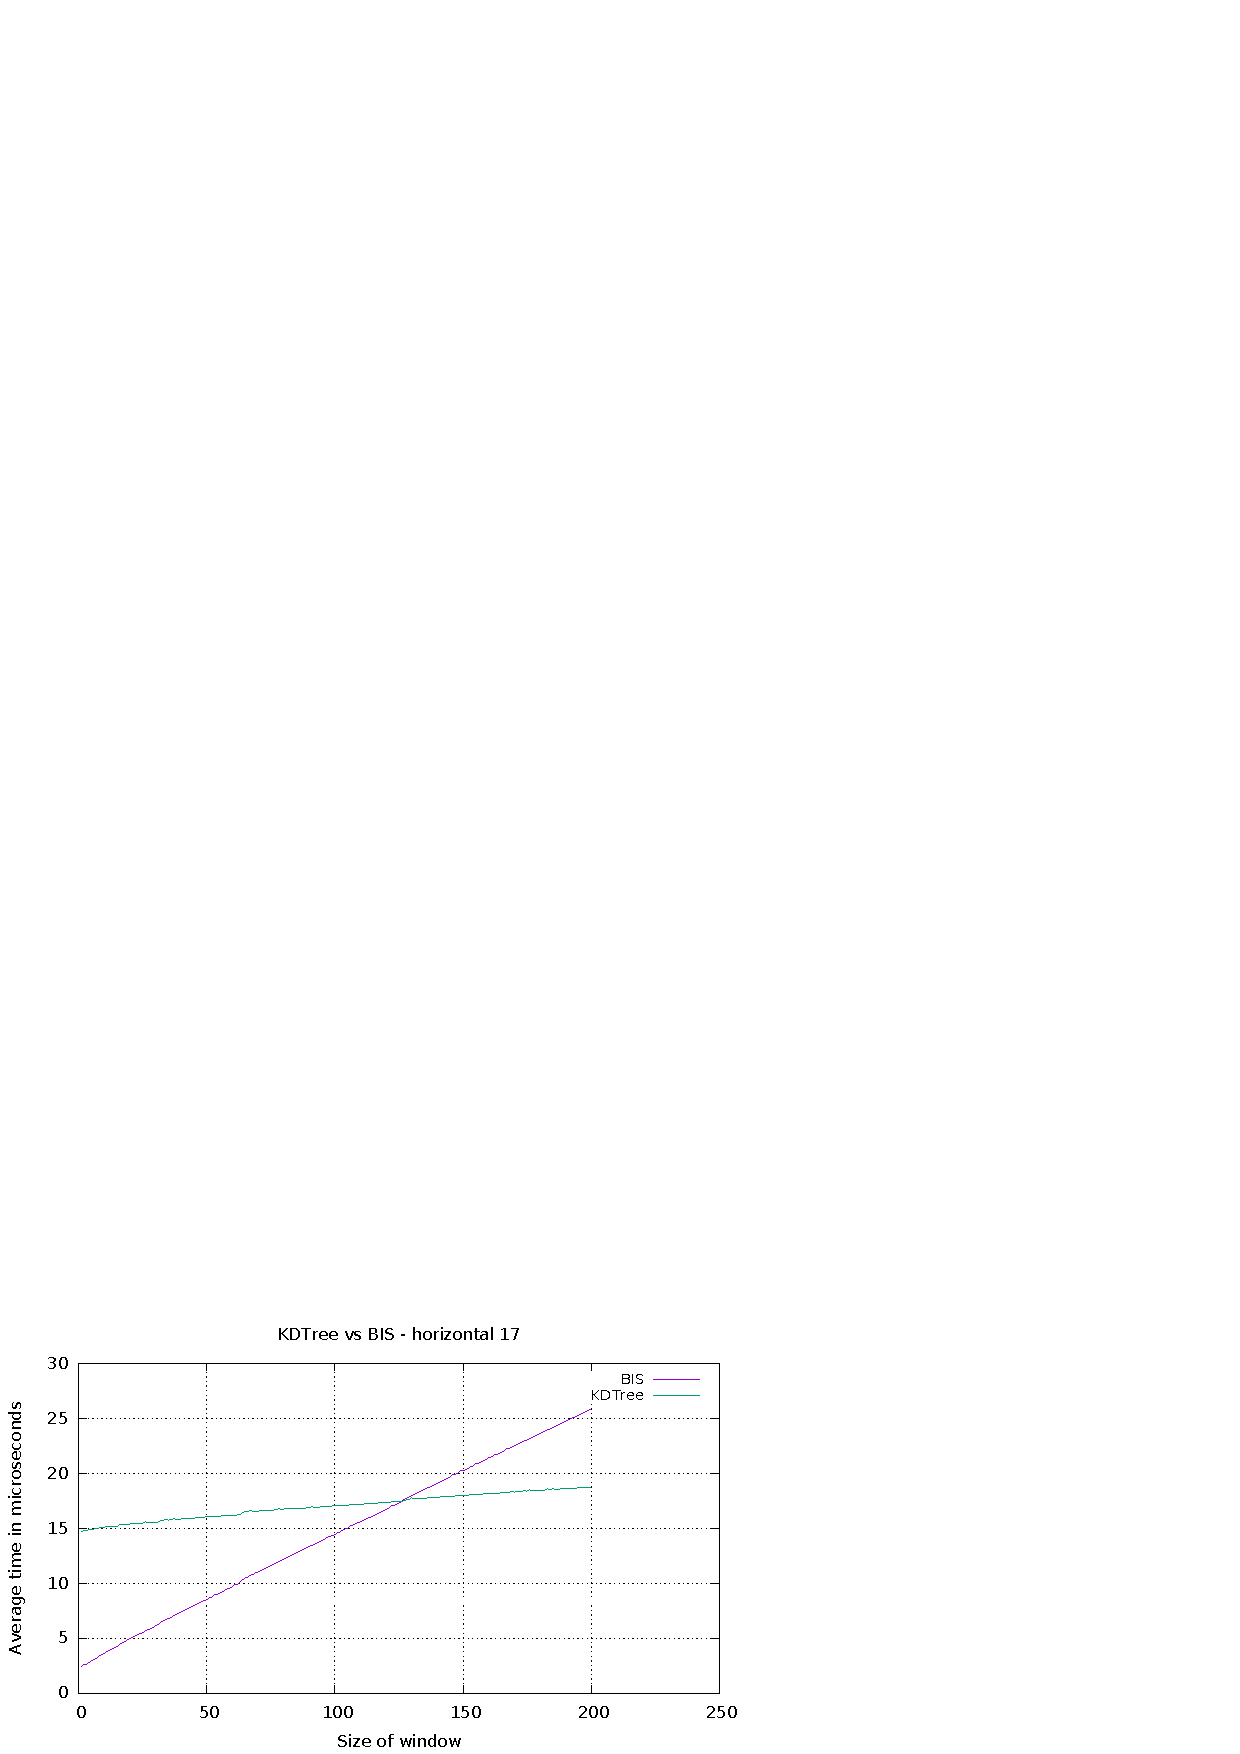
\includegraphics[width=0.99\textwidth]{pictures/analysis/hori_17.png}
        \caption{$n = 2^{17}$}
        \label{fig:hori_17}
    \end{subfigure}
    %\hfill
    \begin{subfigure}[b]{0.68\textwidth}
        \centering
        \includegraphics[width=0.99\textwidth]{pictures/analysis/hori_25.png}
        \caption{$n = 2^{25}$}
        \label{fig:hori_25}
    \end{subfigure}
  }
    \caption{Horizontal slice on BIS and kd-tree.}
    \label{fig:hori_17_25}
  
\end{figure}


To summarize these graphs for horizontal slices, figure~\ref{fig:hori_intersection} shows the size of the slice at the point of intersection between the running-time of a search to the SRS and kd-tree for each $n$ tested. Figure~\ref{fig:hori_intersection} is a little more messy than figure~\ref{fig:vert_intersection} which is a point we will address in section~\ref{sect:verthoriexp}. At figure~\ref{fig:hori_theory} the graph crosses above and below $1$, but keeps rather close to $1$ which is the point where the performance is as we would theoretically expect. Looking at figure~\ref{fig:hori_theory_worst_jump} we see the intersection graph normalized by the worst-case jumps. This always stays above $1$. As we will also address in section~\ref{sect:verthoriexp} we expect the distribution of jumps in a certain way, and depending on where the worst jump, which is level $15$, resides compared to the least common ancestor of $x_1$ and $x_2$ the average jumps per result will change.

\begin{figure}[h]
  \makebox[\linewidth][c]{
    \centering
    \begin{subfigure}[b]{0.68\textwidth}
        \centering
        \includegraphics[width=0.99\textwidth]{pictures/analysis/hori.png}
        \caption{Point of intersection between BIS and kd-tree.}
        \label{fig:hori_intersection}
    \end{subfigure}
    %\hfill
    \begin{subfigure}[b]{0.68\textwidth}
        \centering
        \includegraphics[width=0.99\textwidth]{pictures/analysis/hori_theory.png}
        \caption{Point of intersection normalized by theoretical $k$}
        \label{fig:hori_theory}
    \end{subfigure}
  }
    \caption{Horizontal slice on BIS and kd-tree.}
    \label{fig:hori_intersection_and_theory}
  
\end{figure}
\clearpage

\section{Comparision of SRS and kd-tree with a small $k$}
\label{sect:smallk}


In this section we are going to look at slices with $k\leq 200$. We will only focus on vertical slices. We are interested in seeing how much faster the SRS data structure is than the kd-tree when looking at amounts of results which seems reasonable to user interaction. Figures~\ref{fig:small_hori_17} through ~\ref{fig:small_vert_25} show the performance a search query to the BIS data structure compared to a search query to the kd-tree, where $k \leq 200$ for both horizontal and vertical slices.

\begin{figure}[h]
  \makebox[\linewidth][c]{
    \centering
    \begin{subfigure}[b]{0.68\textwidth}
        \centering
        \includegraphics[width=0.99\textwidth]{pictures/analysis/smalls/vert_17.png}
        \caption{Data set of size $n=2^{17}$.}
        \label{fig:small_vert_17}
    \end{subfigure}
    %\hfill
    \begin{subfigure}[b]{0.68\textwidth}
        \centering
        \includegraphics[width=0.99\textwidth]{pictures/analysis/smalls/vert_25.png}
        \caption{Data set of size $n=2^{25}$.}
        \label{fig:small_vert_25}
    \end{subfigure}
  }
    \caption{Vertical slice on BIS and kd-tree.}
    \label{fig:small_vert_17_25}
  
\end{figure}

The running time of a slice to the BIS data structure where $k \leq 200$ is noticably better than the running time of a slice to the kd-tree. It is only on figure~\ref{fig:small_hori_17} that we see the graphs intersect. All other figures show that the BIS data structure performs better when the size of the slice is below $200$. Seeing this tendency, we are then also interested in testing just how much better the BIS data structure performs. We are going to meassure this by testing the factor between the performance of the BIS data structure and the performance of the kd-tree. We see the result of these tests on figure~\ref{fig:small_hori_fac_17} through ~\ref{fig:small_vert_fac_25}.



\begin{figure}[h]
  \makebox[\linewidth][c]{
    \centering
    \begin{subfigure}[b]{0.68\textwidth}
        \centering
        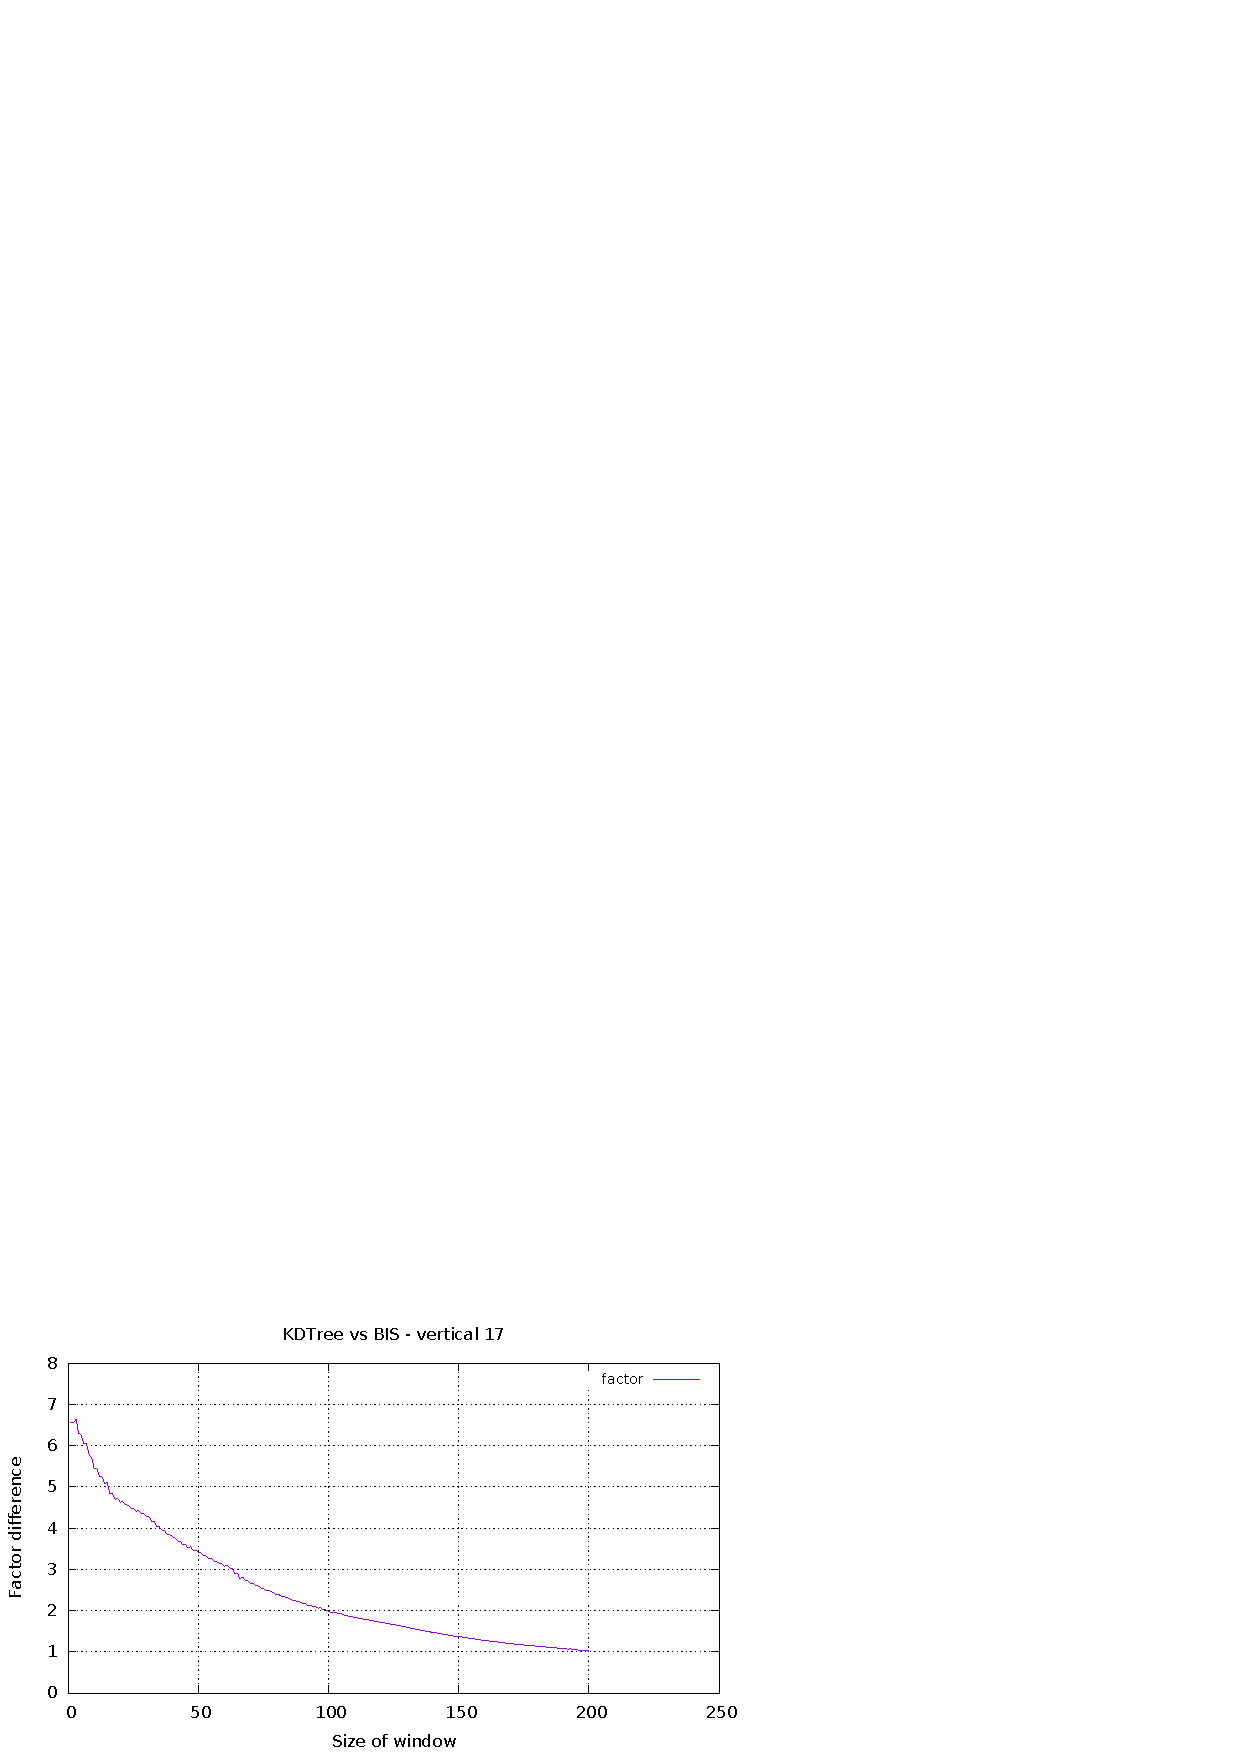
\includegraphics[width=0.99\textwidth]{pictures/analysis/smalls/vert_fac_17.png}
        \caption{Data set of size $n=2^{17}$.}
        \label{fig:small_vert_fac_17}
    \end{subfigure}
    %\hfill
    \begin{subfigure}[b]{0.68\textwidth}
        \centering
        \includegraphics[width=0.99\textwidth]{pictures/analysis/smalls/vert_fac_25.png}
        \caption{Data set of size $n=2^{25}$.}
        \label{fig:small_vert_fac_25}
    \end{subfigure}
  }
    \caption{Ratio between running time of slice on BIS and kd-tree.}
    \label{fig:small_vert_fac_17_25}
  
\end{figure}
\clearpage

Looking at figure~\ref{fig:small_hori_fac_17} and figure~\ref{fig:small_hori_fac_25} we notice that the factor difference at $size=100$ increases from just above $1$ to around $13$. At $\lg n = 25$ a horizontal slice with $size = 100$ is a factor $13$ better than the kd-tree. \todo{Skal jeg lave en graf med det? Sæt size fast og se hvordan faktoren stiger når $\lg n$ vokser?}

Looking at figure~\ref{fig:small_vert_fac_17} and figure~\ref{fig:small_vert_fac_25} the same trend is seen. Looking at $size = 100$ we notice the factor growing from $2$ to $27$. A factor of $27$ is the difference between the vertical slice to the BIS data structure and a vertical slice to the kd-tree with $size = 100$.

Looking back to the section about the square windows we remember that a window with the dimensions $\sqrt{n}\cdot{size} \times \sqrt{n}\cdot\sqrt{size}$ is expected to return $size$ points as result. This was based on the area of area of the search query. Thus, we can rewrite the expression as follows: $\sqrt{n}\cdot{size} \times \sqrt{n}\cdot\sqrt{size} = \sqrt{n}\cdot\sqrt{n} \times \sqrt{size}\cdot\sqrt{size} = n \times size$ which is exactly what vertical or horizontal slice looks like. Thus, we know that these two types of queries are expected to return the same amount of points and we can therefore compare the square search query with a horizontal or vertical slice to see how much of an impact the shape of the search has for the SRS data structure. We could do the same for the kd-tree, but we notice a big difference in the running time between figure~\ref{fig:sqrt_24} and figure~\ref{fig:small_vert_24} and that analysis falls outside the scope of this thesis. We have already seen that there is noticable difference between a horizontal slice and a vertical slice when querying the SRS data structure, but it interesting to see how well the squared query compares to those. 


We pick $size=\{50,100,150\}$ from both the squared tests and the slices to see how changing the shape of the query affects the running time of the query to the SRS data structure. The graphs on figure~\ref{fig:all_50}, figure~\ref{fig:all_100} and figure~\ref{fig:all_150} show some similarities. The vertical slice is clearly the fastest. The horizontal slice performs worse than the vertical slice. The squared window search query seems to be the worst-case scenario for the graphs. But looking at only the squared window search across the three graphs we see that it growing with a rather linear tendency. We would expect as much from the theory because if we fix $k$ in $\mathcal{O}(\lg n + k\cdot \lg^\epsilon n$ we only have $\lg n$ and $lg^\epsilon n$ growing. Since $\lg n$ increases by $1$ and $lg^\epsilon n$ is an expression for the amount of jumps performed, this ties rather well to the theory. Looking at these three graphs, we suspect that the squared window search is the general case of a search query to the BIS data structure, while both the horizontal and vertical slice searches are special cases performing even better. \todo{Det er tydeligt fra teorien - og forklaringen ovenfor - at vertical er det bedste. Hvorfor er horizontal bedre end sqrt?}. Thus, the time required to find $k$ points with a search query to the BIS data structure is bound by a graph growing linearly to $\lg n$. 


\begin{figure}[h]
  \makebox[\linewidth][c]{
    \centering
    \begin{subfigure}[b]{0.68\textwidth}
        \centering
        \includegraphics[width=0.99\textwidth]{pictures/analysis/smalls/all_100.png}
        \caption{Queries to the BIS data structure with $size=100$.}
        \label{fig:all_100}
    \end{subfigure}
    %\hfill
    \begin{subfigure}[b]{0.68\textwidth}
        \centering
        \includegraphics[width=0.99\textwidth]{pictures/analysis/smalls/all_kdtree_100.png}
        \caption{Queries to the kd-tree with $size=100$.}
        \label{fig:all_kdtree_100}
    \end{subfigure}
  }
  \caption{Comparison of shapes on BIS and KDtree.}
  \label{fig:all_100_and_kdtree}
  
\end{figure}

\begin{figure}[h]
  \makebox[\linewidth][c]{
    \centering
    \begin{subfigure}[b]{0.68\textwidth}
        \centering
        \includegraphics[width=0.99\textwidth]{pictures/analysis/smalls/all_50.png}
        \caption{Queries to the BIS data structure with $size=50$.}
        \label{fig:all_50}
    \end{subfigure}
    %\hfill
    \begin{subfigure}[b]{0.68\textwidth}
        \centering
        \includegraphics[width=0.99\textwidth]{pictures/analysis/smalls/all_150.png}
        \caption{Queries to the kd-tree with $size=150$.}
        \label{fig:all_150}
    \end{subfigure}
  }
  \caption{Comparison of shapes on BIS.}
  \label{fig:all_50_and_150}
  
\end{figure}


We look at figure~\ref{fig:all_kdtree_100} in order to confirm changing the shape from a squared window to a vertical or horizontal slice impacts the time of the search query to kd-tree in a much bigger way than changing the shape of the search query to the SRS data structure.

In section\todo{square kapitel} we found the ratio between a square query to the kd-tree and a square query to the BIS data structure in order to find out how much better the kd-tree performed. Now the roles are reversed, and we are now interested in seeing how much better the BIS data structure performs. 


\begin{figure}[h]
  \makebox[\linewidth][c]{
    \centering
    \begin{subfigure}[b]{0.68\textwidth}
        \centering
        \includegraphics[width=0.99\textwidth]{pictures/analysis/factor_difference_vert_50.png}
        \caption{Ratio with $size=50$.}
        \label{fig:fact_diff_vert_50}
    \end{subfigure}
    %\hfill
    \begin{subfigure}[b]{0.68\textwidth}
        \centering
        \includegraphics[width=0.99\textwidth]{pictures/analysis/factor_difference_vert_100.png}
        \caption{Ratio with $size=100$.}
        \label{fig:fact_diff_vert_100}
    \end{subfigure}
  }
  \caption{Ratio between BIS data structure and kd-tree. Describes how much better the BIS data structure performs compared to the kd-tree.}
  \label{fig:fact_diff_vert_50_100}
  
\end{figure}


\begin{figure}[h]
    \centering
    \includegraphics[width = 0.85\textwidth]{pictures/analysis/factor_difference_vert_150.png}
    \caption{Ratio between BIS data structure and kd-tree with $size=150$. Describes how much better the BIS data structure performs compared to the kd-tree.}\label{fig:fact_diff_vert_150}
\end{figure}
\clearpage



\section{Comparison of the different SRS data structures with $B$ varying}

So far we have only looked at the SRS data structure with $B=2$. We have also not yet mentioned the important aspect of how much main memory the SRS data structure uses compared to the kd-tree. In this section we are going to show how much space the SRS data structure with $B={2,3,4}$ uses and compare it to the space used by the kd-tree. We will also look at how well the vertical and horizontal slices perform with $B={3,4}$ by looking at when the query time for a search query to SRS data structure instersects the query time for a search query to the kd-tree. \todo{Måske også kigge på hvordan k-theory-normalization ser ud}


As we briefly looked at in section\todo{ref} another aspect to investigate would be to have a search query of a fixed area performed to both data structures with a growing $\lg n$. However, based on the theory of how many points we expect to find in a given area based on the point-size and area of a data structure, this query would return less and less points. \todo{Er det overhovedet spændende at kigge på? Jeg tænker lidt det bare kommer til at vise det samme vi allerede ved. Med lidt snilde kan vi gøre det med eksisterende data da $\sqrt{2^17}*1.5 = 540$ og $\lg 540 \approx 9$ og $25-17 = 8$. Så vi har nok til at vi kan formindske det nedad.}

We are going to briefly look at how the BIS data structure performs with $B=\{3,4\}$. We start by introducing figure~\ref{fig:b3_vert_intersection} and figure~\ref{fig:b3_hori_intersection} to see at what size the running time of vertical and horizontal slices to the BIS data structure with $B=3$ intersects with the running time of the same query to the kd-tree. Recall we have already seen these graphs for $B=2$ on figure~\ref{fig:vert_intersection} and figure~\ref{fig:hori_intersection}.

We will also check if the intersection point is as we theoretically expect it. Thus, we normalize the time of the intersection with the theoretically expected  $k$. We see the graphs on figure~\ref{fig:b3_vert_theory}, figure~\ref{fig:b3_vert_theory_worst},  figure~\ref{fig:b3_hori_theory} and figure~\ref{fig:b3_hori_theory_worst}.We have also already seen this for $B=2$. 

We are going to introduce the exact same graphs for $B=4$. These are seen on figures~\ref{fig:b4_vert_intersection} through ~\ref{fig:b4_hori_theory_worst}.



\begin{figure}[h]
  \makebox[\linewidth][c]{
    \centering
    \begin{subfigure}[b]{0.68\textwidth}
        \centering
        \includegraphics[width=0.99\textwidth]{pictures/analysis/threes/vert.png}
        \caption{Point of intersection with $B=3$.}
        \label{fig:3vert}
    \end{subfigure}
    %\hfill
    \begin{subfigure}[b]{0.68\textwidth}
        \centering
        \includegraphics[width=0.99\textwidth]{pictures/analysis/fours/vert.png}
        \caption{Point of intersection with $B=4$.}
        \label{fig:4vert}
    \end{subfigure}
  }
  \caption{Ratio between BIS data structure and kd-tree. Describes how much better the BIS data structure performs compared to the kd-tree.}
  \label{fig:34vert}
  
\end{figure}

\begin{figure}[h]
  \makebox[\linewidth][c]{
    \centering
    \begin{subfigure}[b]{0.68\textwidth}
        \centering
        \includegraphics[width=0.99\textwidth]{pictures/analysis/comparing_BIS_50.png}
        \caption{BIS with $size = 50$.}
        \label{fig:BIS_50}
    \end{subfigure}
    %\hfill
    \begin{subfigure}[b]{0.68\textwidth}
        \centering
        \includegraphics[width=0.99\textwidth]{pictures/analysis/comparing_BIS_100.png}
        \caption{BIS with $size = 100$.}
        \label{fig:BIS_100}
    \end{subfigure}
  }
  \caption{BIS with $B = \{2,3,4\}$. Comparing vertical slices to each}
  \label{fig:comparing_BIS}
  
\end{figure}


The most important reason why the range tree is not used as the standard range reporting data structure today is its space complexity. While we have shown theoretically that the space complexity of the BIS data structure is linear, we would also like to see it in practice. Figure~\ref{fig:sizes} shows the actual space usage of the BIS data structure with $B=\{2,3,4\}$ and the space usage of the kd-tree. The size has been normalized by the amount of points the data structure holds. Thus, the normalized size of the kd-tree is $2$, meaning that for each point in the kd-tree it uses $2\cdot 32$ bits - one $32$ bits integer for each coordinate.

\begin{figure}[h]
    \centering
    \includegraphics[width = 0.85\textwidth]{pictures/analysis/sizes.png}
    \caption{The normalized sizes of the BIS data structure with $B=\{2,3,4\}$ and the kd-tree.}\label{fig:sizes}
\end{figure}

\clearpage


\section{Vertical and horizontal slices explained}
\label{sect:verthoriexp}

In this we are going to dive a deeper into the results of the previous section. The figures depicting the performance of the vertical slices showed some interesting tendencies. This is the main focus of this section.

\begin{figure}[h]
    \centering
    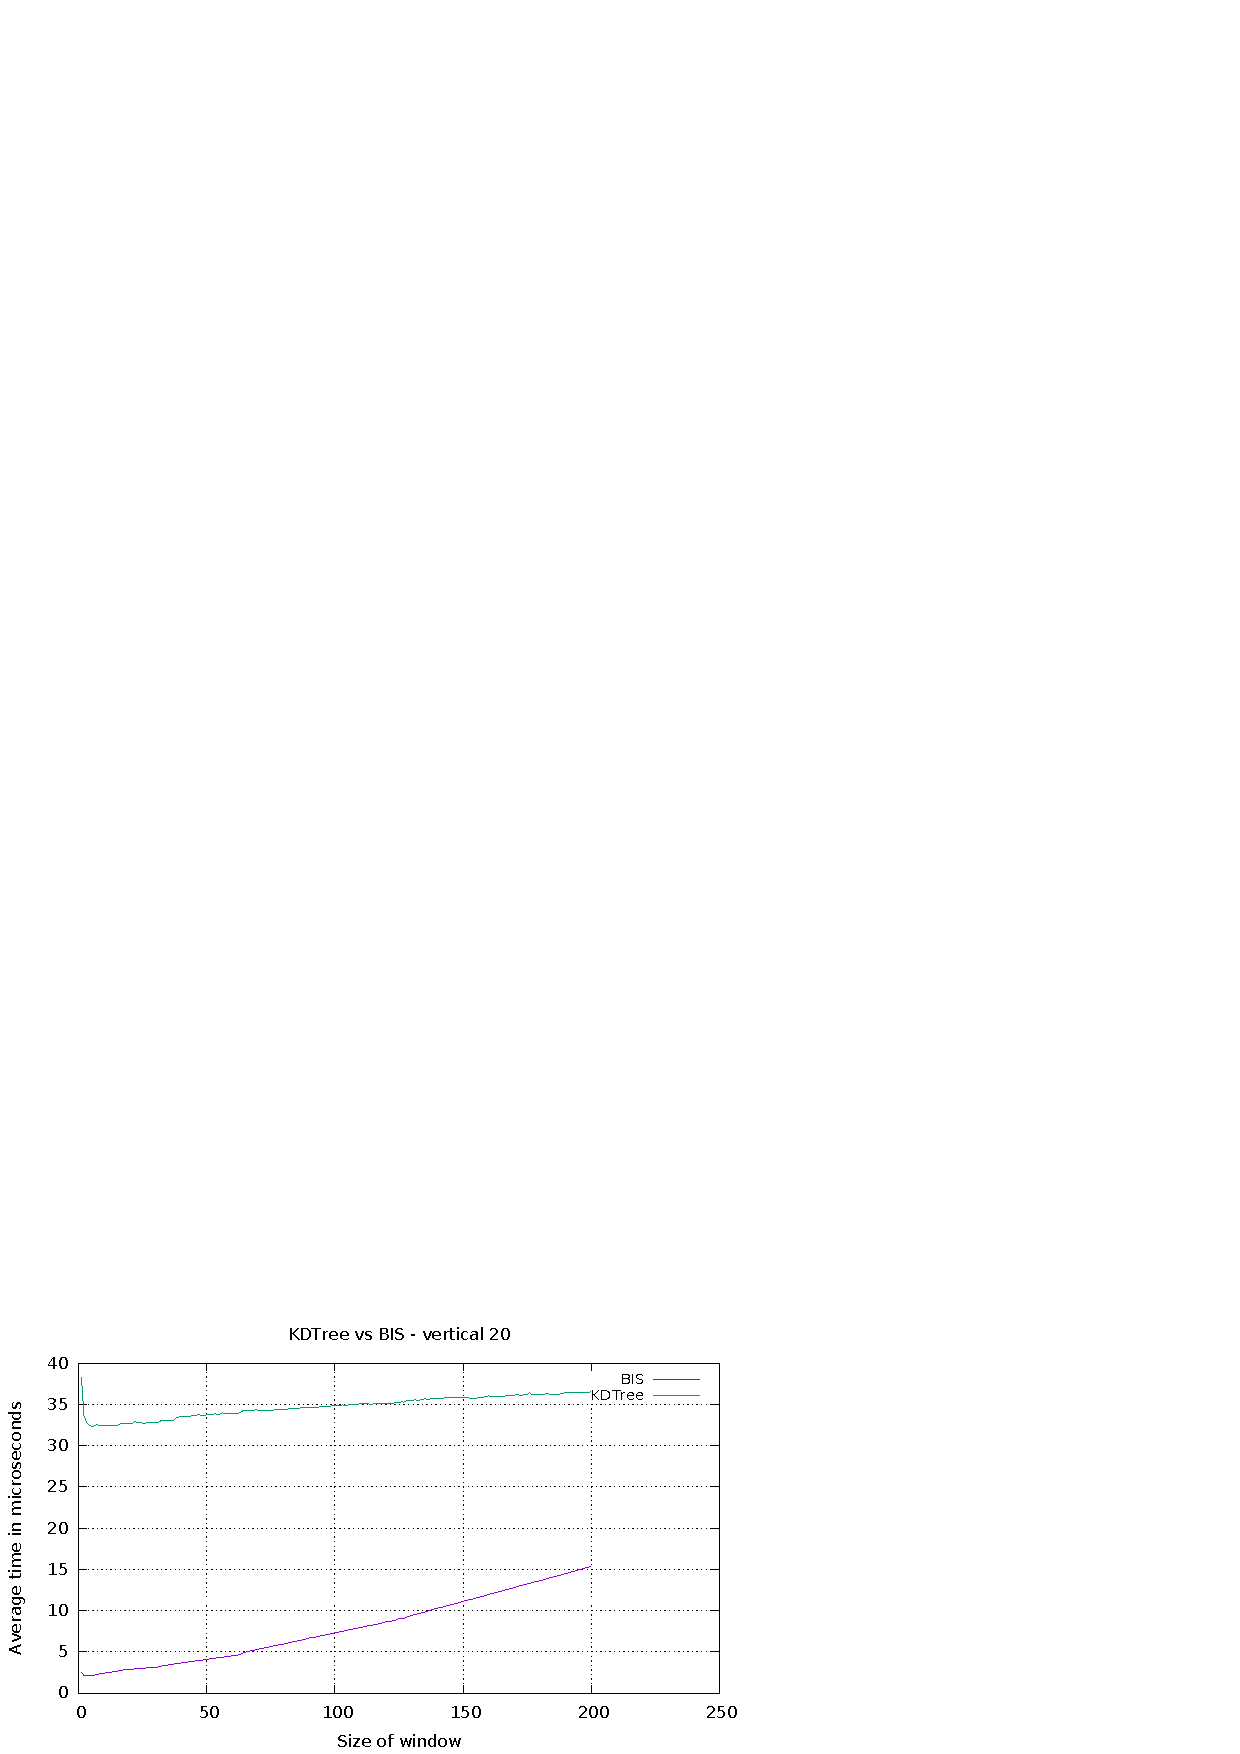
\includegraphics[width = 0.85\textwidth]{pictures/analysis/vert_20.png}
    \caption{Vertical slice. data set size of $n=2^{20}$.}\label{fig:vert_20}
\end{figure}



\begin{figure}[h]
    \centering
    \includegraphics[width = 0.85\textwidth]{pictures/analysis/jump_vert_17.png}
    \caption{Size of jumps - data set size of $n=2^{17}$. 'Average jumps' is the average of all the jumps performed normalized by the size of the slice}\label{fig:jump_vert_17}
\end{figure}

\begin{figure}[h]
    \centering
    \includegraphics[width = 0.85\textwidth]{pictures/analysis/jump_vert_20.png}
    \caption{Size of jumps - data set size of $n=2^{20}$. 'Average jumps' is the average of all the jumps performed normalized by the size of the slice}\label{fig:jump_vert_20}
\end{figure}



\begin{figure}[h]
    \centering
    \includegraphics[width = 0.85\textwidth]{pictures/analysis/level_vert_17.png}
    \caption{Level of first fully contained node - data set size of $n=2^{17}$.}\label{fig:level_vert_17}
\end{figure}

\begin{figure}[h]
    \centering
    \includegraphics[width = 0.85\textwidth]{pictures/analysis/level_vert_20.png}
    \caption{Level of first fully contained node - data set size of $n=2^{20}$.}\label{fig:level_vert_20}
\end{figure}


Across the graphs showing the performance of the vertical slices to the BIS data structure, there is a very noticable change in slope at around $k=256$. Since $B=2$, we have a big jump at level $2^3 = 8$ which allows the ball inheritance structure to jump from level $8$ to a leaf in one jump. This means that the average amount of jumps per result will decrease and thus the running time will not increase as fast as before. At around $k=512$ the running-time resumes its normal behaviour. On average, the ball inheritance structure does not use the big jump at level $8$ directly anymore, resulting in a couple of steps before reaching level $8$. Since the graph shows the average run-time of different configurations of the same slice on different data sets, not all of the searches will hit level $8$ from $k>256$, but the main tedency is to. \todo{forklar tidligere - at vi snakker om main tendency, ikke hvad den er garanteret at gøre}. This tendency is described at figure~\ref{fig:jump_vert_17} and figure~\ref{fig:jump_vert_20}. We see how the graph has a local maximum at around $k=256$ and then the average amount of jumps per result decreases until $k=512$ where it starts increasing at steady level again. Figure~\ref{fig:level_vert_17} and figure~\ref{fig:level_vert_20} describes the highest level of a fully contained node. We see between $k=256$ and $k=512$ that the maximum is level $8$ and the minimum is level $7$ and that the average level increases meaning more and more fully contained node starts using level $8$. Since we $B=2$, there is a $2$-jump every $2$ levels, a $4$-jump every $4$ levels, a $8$-jump every $8$ levels and a $16$-jump every $16$ levels. This means that level $7$ the ball inheritance structure needs $3$ jumps to reach a leaf. This is why such a noticable local maximum exits on figure~\ref{fig:jump_vert_17} and figure~\ref{fig:jump_vert_20}. The jumps per results eases off because from level $8$ there is $1$ jump, from level $9$ there are $2$ jumps and from level $10$ there are $2$ jumps. Levels $11, 13, 14$ have $3$ jumps, and at level $15$ another local maximum is going to be found with $4$ jumps, just before level $16$ with $1$ jump to the leaves. However, $k=2^{16}=65,536$ is not likely to be a place where the SRS data structure performs better than the kd-tree unless we have a enormous data set \todo{regn på det}. \todo{Sæt grafer ind for større $n$}


Looking at figure~\ref{fig:level_vert_17} we see that when we reach $k=256$ the minimum highest level rises to $7$ and the maximum highest level rises to $8$. In order to write the sum of $256<k<512$ we will need to at least level $7$ because we need the two fully included nodes from level $7$ giving us $2*2^7 = 2^8 = 256$ nodes. If the least common ancestor is found at level $9$ the first fully contained node can be found at level $7$. If all the levels from level $7$ to level $1$ only have fully contained nodes, we get $k = 2*2^1 + 2*2^2 + \cdots + 2*2^7 = 508$. This is not enough to write $512$, and thus somewhere between $k=256$ and $k=512$, the search algorithm will begin using level $10$ as the least common ancestor. This is also very dependent on how the slice covers the subtrees of the least common ancestor. If the slice hits the least common ancestor right in the middle, such that the left subtree and the right subtree of the least common ancestor is of the exact same size, the level of the highest fully included node will be lower. If the slice hits the least common ancestor such there is an imbalance in the size between the left subtree and right subtree of the least common ancestor, the level of the highest fully included node will be higher, because now one subtree has to account for a bigger portion of the slice and will have to use bigger pieces. And when a subtree contains $2^8 = 256$ leaves it will have access to the jump at level $8$. The maximum level of figure~\ref{fig:level_vert_17} is explained by the fact that it is not possible to write the sum of $k<512$ using $512$ as a summand. Recall that a vertical slice conceptually only searches for the x-coordinates of the points. All the y-coordinates are already known to be included, Thus, when a node is fully included, we get all of points in its subtree.   \todo{Omformuler og sæt sammen med afsnittet fra før lige ovenover da du skriver nogenlunde det samme - bare i to forskellige tankegange}\todo{Lav en lignede figur som figur 3.2 til at forklare konceptet}

As mentioned before, it is hard to argue about the tendencies of the graphs of the horizontal slices. When the least common ancestor of $x_1$ and $x_2$ is found at level $i$, the first node which is fully contained in a horizontal slice is located on level $i-2$. So from level $i-1$ to level $1$ we find $2$ fully contained nodes per level. The points are uniformly distributed which means that given one y-rank the chance to find it on level $i-2$ is $2\cdot\frac{1}{4} = \frac{1}{2}$. The chance to find it on level $i-3$ is half that, i.e. $\frac{1}{4}$. Thus, when we see the graphs of the horizontal slices.. bla bla

\begin{figure}[h]
    \centering
    \includegraphics[width = 0.85\textwidth]{pictures/analysis/jump_hori_17.png}
    \caption{Size of jumps - data set size of $n=2^{17}$. 'Average jumps' is the average of all the jumps performed normalized by the size of the slice}\label{fig:jump_hori_17}
\end{figure}
\clearpage

Forklar konceptet med hvordan average jumps ser ud. This seemingly uninteresting graph shows us that the theory of the expected distribution is correct. We also had this confirmed in section~\ref{sect:squares} where we saw that square searches of size $\sqrt{n}\cdot\sqrt{k} \times \sqrt{n}\cdot\sqrt{k}]$ returned $k$ results. This was based on theory that assumed the distribution was uniform. If the y-coordinates are uniformly distributed amongst the x-coordinates to generate a point, we can see something interesting in figure~\ref{fig:jump_hori_17}. A BIS data structure with data set size $n = 2^{17}$ will have its first fully contained node at level $15$. For each y-coordinate we have to find, there is a $\frac{2}{4} = \frac{1}{2}$ chance that it will jump from level $15$. Then there is a $\frac{1}{4}$ chance that it will jump from level $14$ and so on. Given this information we can we can use table-something to see how many jumps a ball must take in order to get from a node at level $i$ to a leaf. Doing this we see that $\frac{4}{2} + \frac{3}{4} + \frac{3}{8} + \frac{2}{16} + \frac{3}{32} + \frac{2}{64} + \frac{2}{128} = 3.391$ which is the jumps per results depicted on figure~\ref{fig:jump_hori_17}. \todo{Kan jeg nu rent faktisk bruge det her til at forklare hvor hori tager de mærkelige svingninger?}

SENERE: Kig på $size = 300$ for alle $\lg n$. Se hvordan det er dårlig ved $\lg n = 17$ for der er første hop med størst sandsynlighed på level 15 som er $1+2+4+8 = 15 => 4$ hop. Ved $\lg n = 18$ er den god for der er størst sandsynlighed for $16 => 1$ hop. Når vi kommer højere f.eks. $\lg n = 24$ er første hop ved level $22 = 2 + 4 + 16$ og andet hop er $1 + 4 + 16$. Så tre hop er $\frac{3}{4}$ sandsynlighed. Sammenlign det med en hvor der er $2$ og $3$, f.eks. $\lg n = 22$.
\todo{Forklar om hvordan distribution af points og hvordan hvor vi ligger i forhold til level $15$ betyder noget. Kig også på grafen for figur~\ref{fig:hori_jumps_per_lgn}. Den viser netop at $\lg n = 17$ med LCA = level $15$ er noget skidt.}


\todo{Hvorfor knækker grafen mellem $512$ og $1024$? Hvorfor er kd-træet mærkeligt dårligt inden $k=10$? HORI}





\section{Summary}

In this chapter we have presented different tests on the BIS data structure. We have compared it to the kd-tree and confirmed that the theory works well in practice.

The BIS data structure performs very well as a slice, most notably as a vertical slice. A square search query does not perform as well as a slice does on the BIS data structure. Howeve the square search query is not a disaster on the BIS data structure. We noticed the difference in performance between the square and slice-formed search query to the BIS data structure was not as big as the difference in performance between the two shapes on the kd-tree. The worst kind of test for the kd-tree was a slice and the best was a square - the exact opposite of the BIS data structure.

The kd-tree is much more dependent on the shape of its search query than the BIS data structure. This is most notable by looking at the difference between figure~\ref{fig:all_100} and figure~\ref{fig:all_kdtree_100}.


En spændende sammenhæng. Hvor kd-træet er dårlig er BIS god, og omvendt. kd-træet er dog stadig kun præcis lineær i tid, men BIS har en penalty pr point. Men i små punkt-mængder er BIS rent faktisk rigtig god. Forskellen mellem shapes er ikke så drastisk som kd-træet.

Hvordan adskiller de forskellige shapes sig i SRS? Vi ser at kd-træet er meget afhængig af sin shape i praksis som den er i teori. Hvordan gælder det for SRS? Hvordan adskiller de forskellige shapes fra hinanden tidsmæssigt? 


\chapter{conclusion}
\label{ch:conclusion}

Something something


%%%%%%%%%%%%%%%%%%%%%%%%%%%%%%%%%%%%%%%%%%%%%%%%%%%%%%%%%%%%%%%%%%%%%%%

\addcontentsline{toc}{chapter}{Primary Bibliography}
\bibliographystyle{plainnat} 
\bibliography{refs}

\end{document}

